

% For Stacey to use in place of JIBLM.tex.  Removed identification of JIBLM.

\documentclass[oneside]{book}
\usepackage{enumerate}
\usepackage{amssymb}
\usepackage{amsmath}
\usepackage{latexsym}
\usepackage{amsthm}
\usepackage{mathptmx}
\usepackage{verbatim}
\usepackage{endnotes}
   

\usepackage{fancyhdr}
\pagestyle{fancy}

\renewcommand{\chaptermark}[1] {\markboth{#1}{}}%

\setlength{\oddsidemargin}{63pt}
\setlength{\evensidemargin}{63pt}

\setlength{\parskip}{1mm}
\setlength{\textwidth}{5.0in}
\setlength{\textheight}{8.5in}
\let\affiliation\date

\makeatletter
\def\maketitle{%
  \null
  \thispagestyle{empty}%
%%%%%%%%%%%%%%%%%%%%%%%%%%%%%%%%%%%%%%%

  \normalfont
  \vspace{2in}
\begin{center}\leavevmode
{\Huge \@title\par}%
\vspace{20mm}
{\Large \@author\par}%
\vspace{5mm}
{\Large \@date\par}
{\Large \ }
\end{center}
  \vfill
  \null
  \cleardoublepage
 \let\newauthor\@author
 }%
\makeatother

\lhead{ \leftmark} \chead{} \rhead{\thepage}
\renewcommand{\headrulewidth}{0.4pt}
\usepackage{comment}
\newcommand{\InstructorVersion}{\includecomment{annotation}}
\newcommand{\StudentVersion}{\excludecomment{annotation}}

\makeatletter
\renewcommand{\@makechapterhead}[1]{%
\vspace*{50\p@}%
  {\parindent \z@ \raggedright \normalfont
    \ifnum \c@secnumdepth >\m@ne
      \if@mainmatter
        \huge \@chapapp\space \thechapter                
        \par\nobreak
        \vskip 20\p@
      \fi
    \fi
    \interlinepenalty\@M
    \LARGE\bfseries  #1\par\nobreak                        
    \vskip 40\p@
  }}

\renewcommand{\@makeschapterhead}[1]{%
  \vspace*{50\p@}%
  {\parindent \z@ \raggedright
    \normalfont
    \interlinepenalty\@M
    \LARGE\bfseries  #1\par\nobreak                      
    \vskip 40\p@
  }}

\makeatother

\newtheorem{theorem}{Theorem}


\usepackage{graphicx}



\theoremstyle{definition} 
\newtheorem*{defn}{Definition}
\newtheorem*{pyth}{Pythagorean Theorem}

\theoremstyle{definition}
\newtheorem{myexa}{Exercise}

\theoremstyle{definition}
\newtheorem{myexb}{Exercise}

\theoremstyle{definition}
\newtheorem{myexc}{Exercise}

\newcommand{\bd}[1]{\textbf{#1}} 
\newcommand{\oq}[4]{\ensuremath{({#1},{#2},{#3},{#4})}}
\newcommand{\ot}[3]{\ensuremath{({#1},{#2},{#3})}}
\newcommand{\op}[2]{\ensuremath{({#1},{#2})}}
\newcommand{\vect}[1]{\ensuremath{\mathbf{#1}}}
\newcommand{\mtx}[1]{\ensuremath{\texttt{#1}}}

\setcounter{endnote}{-1}

%%%%%%%%%%%%%%%%%%%%% Annotation Environment Switch%%%%%%%%%%%%
\StudentVersion
%\InstructorVersion
%%%%%%%%%%%%%%%%%%%%% Annotation Environment Switch%%%%%%%%%%%%
%


\begin{document}
\large
\frontmatter
\title{Introduction to Linear Algebra}
\author{}
\affiliation{}
\maketitle
\tableofcontents








%%%%%%%%%%%%%%%%%%%%%%%%%%%%%%%%%%%%To the Instructor%%%%%%%%%%%%%%%%%%%%%%%%%%%%%%%%

\begin{annotation}
	
\chapter{To the Instructor}
Students who take our Linear Algebra course have been introduced to proof in a discrete math course, but this is their first proof intensive class. I have organized the notes so students can focus on one theorem at a time, with accompanying computational exercises to provide hints, direction and familiarity with new concepts. Once I realized I needed to tell students specifically that the main goal of the course is for them to gain the important skill of "teaching themselves," student response has been very positive.

The notes begin in the familiar world of real 3-dimensional space where students solve systems of equations and are introduced to the key ideas of existence and uniqueness. The second chapter introduces general linear spaces, focusing on the importance of carefully making and using definitions. The second chapter culminates with the definition of dimension.  The final chapter returns to real n-space to complete the course by defining matrices and matrix operations. In this chapter students figure out how the elementary row operations they used for solving systems of equations can be thought of as multiplication by a sequence of elementary matrices. The determinant is defined and shown to capture information about those operations which allows students to prove a simplified version of the standard Linear Algebra  theorem identifying  equivalent statements.  

I am sure there are lots of ways to use these notes. In my course the students are given four different learning tasks:  doing exercises, proving theorems, presenting their proofs and reflecting on their progress. 

The exercises are computational and help the students understand the concepts they will need for each days proof.  Students should come to class each day with the current day's exercises done. Their understanding can be checked and reinforced with a brief quiz or a class discussion. I have used the open source homework system WeBWorK to create on-line versions of the questions which I would be happy to share. 

The students are then ready to begin the proof that follows those exercises. I put the students in groups of 3-4 and have them work at the board. Their first goal is to understand the statement of the theorem and what "shape" the proof might have: direct, contradiction or contrapositive. For each type of proof the students identify what they would need to assume and what would need to be shown. The proofs get more difficult as the course progresses. Comments specific to each proof can be found in the section titled "Notes to the Instructor" at the end of this document. After class the students individually produce a typed up proof of the day's theorem and turn it in so that I can comment on it before the next class period. I use the learning platform, Moodle, but this could also be done over email or with paper copies. Typesetting is minimal, mostly requiring only superscripts and subscripts so programs such as Microsoft Word are sufficient. 


The next day the students return to their groups from the previous day and combine their efforts to put their best version of the proof on the board. I walk around the room answering questions and helping identify possible issues. I then select one group and one person from that group to present to the class and take questions. Students whose group is not selected to present in a given week come to my office to present a proof from that week individually. 

Once a week students add to their reflection journal. I have them do this as a Moodle assignment, but it could be done in paper notebooks. They identify which course goal: problem solving, communication, evaluating arguments, or understanding fundamental principles, they feel they made the most progress on that week. During the course I point out when I see a student making progress in one of these areas and suggest it as a good journal entry. This reflection helps students identify and appreciate the progress they are making. As long as their weekly entry clearly identifies a course goal and specifies what activity led to their progress in that area they get full credit. Some write only one sentence, others much more.   

Motivation for success is built into the structure of the course. Reading the notes and doing the exercises before class means that the student will get farther on the days proof while in class and be more prepared to type it up after class. A well organized and clearly written proof will get better feedback for the next day. Students are motivated to pay attention and ask questions of the person presenting because they can turn in corrections and regain half the points they may have lost on their proof. Students are required to present one proof each week. They can accomplish this by coming to my office and presenting their choice of one of the most recent 3 proofs. If their group is chosen to present in class, that presentation counts for all group members. This motivates the students to not only prepare good proof presentations, but also to make sure it is well understood by all group members. I allow plus or minus one week of flexibility on when students present. This means if they have already presented and their group is chosen, the group presentation can count for the next week. It also means that if they have a particularly busy week they can miss a presentation and present two times during a later week.

Bookkeeping can be an issue. The daily exercise sets are worth 3 points with no late problems accepted. Students earn 1 point for each problem done. Theorems must also be turned in on time for a score out of 5 points, but then corrections can be submitted one week later where students can earn half the points lost. Students earn 2 points for just restating the theorem, 3 for correctly identify what needs to be assumed and what needs to be shown demonstrating an understanding of any terms used. 4 points if they have one major error or two minor ones and 5 points for a nearly perfect proof. If there is a challenge problem it is only graded if a student's proof is perfect and can earn them 1 extra credit point. Student presentations are 5 points each. Students earn 4 or 5 points, or 0 points with the chance to redo. Each week's reflection is worth 3 points.  

I typically teach 2 sections of 20 students each year and find the grading to be manageable since the student's proofs are typed and corrections are generally good since they are due after we have discussed the proof as a class. The class adapts well for a variety of ability levels. Some students focus on setting up the proofs and understanding the definitions, and often don't have a perfect proof until after they have seen it presented in class. Other students strive to get all of proofs and the Challenge problems. 

We have thirty seven 75 minute long class periods. I found it worked well for each class period to have three parts.  First students would work in small groups to put the key steps of the most recently turned in proof on the board. Then I have one person present. After talking about the presented proof we would move on and make sure everyone understands the definitions and problems for that day. During the last part of the class the students begin to work on proving the next theorem. 

At the beginning of the term I use the Pythagorean Theorem as a low stress introduction to how the class will work. Day one the students brainstorm in groups, with guidance from me. There are several proofs that need only basic geometry and a hint in the form of a picture to get them started.  On the second day students work in small groups and put their proofs of the Pythagorean Theorem on the board.  I help them focus on organizing their board work, justifying each step and introducing their theorem to the class. We then move on to talk about the first three exercises after which the class is ready to begin working in small groups on Theorem\,1.




\end{annotation}


%%%%%%%%%%%%%%%%%%%%%%%%%%%%%%%%%%%%To the Student%%%%%%%%%%%%%%%%%%%%%%%%%%%%%%%%

\chapter{ To the Student}

The main goal of this course is to increase your ability to read and understand new mathematics, connect concepts to justify new statements, and express your reasoning clearly both orally and in writing.  The problems and theorems in these notes carefully build on each other, increasing in content and difficulty. Notice this text is very short compared to most math texts, it is important that you read it carefully and repeatedly.  It is essential that you struggle with each new idea in turn, finding your own solution and not seeking out existing solutions from other texts, on-line sources, or written work done by other students. Talking to other students is encouraged, but only seek out other students once you have made as much progress on the exercises and theorem for yourself as you can. 



\mainmatter





\chapter{Euclidean Space}  \label{Euclidean Space}

\section{Ordered Triples}      \label{Ordered Triples}


\begin{defn}
	An \bd{ordered triple} of real numbers is written $\vect{v}=\ot{v_1}{v_2}{v_3}$ where $v_1$, $v_2$, $v_3$ $\in \mathbb{R}$. Such a triple can be interpreted geometrically as either a point: indicating a position in 3 dimensional space, or as a vector: visualized as an arrow indicating direction which can occur at any position.
	\\
	\\
	Unless otherwise indicated, the Cartesian coordinate system, also known as the rectangular coordinate system, will be used. In this system the x,y and z axis are perpendicular and indicate the direction for the first, second and third coordinates respectively.\\


	\begin{picture}(100,80)(-150,-50)
	\thicklines
	\put(0,-10){\vector(0,1){50}}
	\put(0,-10){\vector(-1,-1){30}}
	\put(0,-10){\vector(1,0){50}}
	\put(-30,-25){x}
	\put(50,0){y}
	\put(-15,30){z}
	\end{picture}
\\	
	As a \bd{point} in the Cartesian coordinate system, $\vect{v} = \ot{v_1}{v_2}{v_3}$, is the position reached by beginning where the axes meet and moving a distance of $v_{1}$ in the x direction, then $v_2$ in the y direction followed by $v_3$ in the z direction.
\\
\\
	As a \bd{vector} in the Cartesian coordinate system, $\vect{v} = \ot{v_1}{v_2}{v_3}$, is visualized as an arrow which can start at any position and ends at the point obtained by moving a distance of $v_1$  in the x direction, then $v_2$  in the y direction followed by $v_{3}$ in the z direction.
\end{defn}

Ordered triples can represent physical concepts such as position, velocity or force. They can also represent any triple of related data such as population of three related species: mice, smakes and hawks, or three related physical properties: temperature, pressure and volume.

\begin{defn}
	The set of all ordered triples is called \bd{Euclidean space} or \bd{real 3-space}, and written: $\mathbb{R}^3$. Using set notation it is written: \[ \mathbb{R}^3=\{\ot{v_1}{v_2}{v_3} | v_1,v_2,v_3 \in \mathbb{R}\} \] 
\end{defn}

\begin{defn}
	Let $\vect{v}=\ot{v_1}{v_2}{v_3} \in \mathbb{R}^3$. The \bd{norm}, also called \bd{length} or the \bd{magnitude} and denoted $\|\vect{v}\|$, is the distance of the point from the origin when \vect{v} is interpreted as a position and the length of the arrow when \vect{v} is interpreted as a vector.
\end{defn}

\begin{pyth}
	For any right triangle with sides of length $a$ and $b$ and hypotenuse $c$: \[a^2+b^2 = c^2\]
\end{pyth}
\vspace{-.3in}\hspace{5in}\begin{annotation}
	\endnote{ When students work on proving the Pythagorean Theorem in class I tell them to use their knowledge of Geometry and give them one of three pictures to work with. From easiest to hardest, the picture hints I find work best are:
			\[ \begin{array}{ccc}
		
\includegraphics[width=0.2\linewidth]{Pyth2} &
		
\includegraphics[width=0.3\linewidth]{Pyth1}&
\includegraphics[width=0.3\linewidth]{Pyth3}
		\end{array} \]  }
\end{annotation}

\begin{myexa}[\bd{a}]
	{Give geometric representations of the points \vect{v} = \ot{3}{-4}{0} and \vect{w} = \ot{3}{-4}{2} using both point and vector interpretations. }
\end{myexa}

\begin{myexb}[\bd{b}]
	{For \vect{v} = \ot{3}{-4}{0} and \vect{w} = \ot{3}{-4}{2} find $\|\vect{v}\|$ and $\|\vect{w}\|$. Show and justify each step.}
\end{myexb}

\begin{myexc}[\bd{c}]
	{Consider an ordered triple $\vect{v}=\ot{v_1}{v_2}{v_3}$, with $\|\vect{v}\|=10$. Does there exist such a \vect{v}?  If so, is \vect{v} unique?  In other words is there exactly one such \vect{v}? }
\end{myexc}

\begin{theorem}
	Let $\vect{v}=\ot{v_1}{v_2}{v_3}$ where $v_1$, $v_2$, and $v_3$ are arbitrary real numbers. The norm of \vect{v} is given by the formula:
	 \[ \|\vect{v}\|= \]
\end{theorem}
\vspace{-.3in}\hspace{5in}\begin{annotation}
	\endnote{Proofs are about justifying your claims. This is a good place to emphasise justifying each step. Some students will already know the distance formula and many will intuitively "know" the triangles formed by moving to the point \vect{v} are right triangles; encourage them to back up these claims by citing definitions and theorems from the text. Once a student gets the big idea, challenge them to consider cases where components are negative or zero. }
\end{annotation}

	
\noindent \textbf{Challenge 1.}  In the case $\vect{v}=\ot{v_1}{v_2}{v_3}$ is interpreted using spherical or cylindrical coordinates the norm of \vect{v} is given by the formula: 
\begin{tabbing}
\indent   i. \space  \= $ \|\vect{v}\|_{spherical}  = $ \\
\indent  ii. \> $ \|\vect{v}\|_{cylindrical}  =$  \\
\end{tabbing}


\section{Vector Operations}      \label{Vector Operations}

\begin{defn}
	Let $\vect{v}=\ot{v_1}{v_2}{v_3}$  and $t \in \mathbb{R}$. The \bd{ scalar product} of $t$ and \vect{v} is defined by: $t\vect{v} = \ot{tv_1}{tv_2}{tv_3}$
\end{defn}

\begin{defn}
   		Let $\vect{v}=\ot{v_1}{v_2}{v_3}$  and $\vect{w}=\ot{w_1}{w_2}{w_3}$. The \bd{sum} of \vect{v} and \vect{w} is defined by: $\vect{v}+\vect{w} =\ot{v_1+w_1}{v_2+w_2}{v_3+w_3}$.  
\end{defn}

These are algebraic definition. It is also important to understand how these definitions affect vectors geometrically. 

\begin{myexa}[\bd{a}]
	Use the vector \vect{v} below and give geometric representations of the vectors described by the scalar products: $3\vect{v}$ and $-1\vect{v}$.\\
		\begin{picture}(100,60)(0,0)
		\thicklines
		\put(130,10){\vector(3,1){100}}
		\put(170,35){\vect{v}}
		\end{picture}
		
\end{myexa}

\begin{myexb}[\bd{b}]
    Given $\vect{v} = \ot{1}{-2}{2}$, find a vector with the same direction as \vect{v}, but with length $1$, with length $10$, and with length $h$.
\end{myexb}

\begin{myexc}[\bf{c}]
	Use the vectors \vect{v} and \vect{w} below to give a geometric representation of the vector which is the sum $\vect{v}+\vect{w}$. If this interpretation is applied to \vect{w}+\vect{v} is the result the same? If this interpretation is applied to $(\vect{v} +\vect{w}) + \vect{u}$  and $\vect{v} + ( \vect{w} + \vect{u})$  are those results the same? \\	
		\begin{picture}(100,60)(0,0)
		\thicklines
		\put(20,10){\vector(3,1){100}}
		\put(200,10){\vector(0,1){30}}
		\put(310,10){\vector(-1,1){40}}
		\put(60,35){\vect{v}}
		\put(210,30){\vect{w}}
		\put(300,35){\vect{u}}
		\end{picture}
 \end{myexc}
 
\begin{theorem}
 	For any ordered triple \ \  $\vect{v}=\ot{v_1}{v_2}{v_3} \in \mathbb{R}^{3}$ \ \ there exists an  ordered triple $\vect{x}=\ot{x_1}{x_2}{x_3} \in \mathbb{R}^{3}$  such that when \vect{x}  is added to \vect{v} the result is the \bd{origin}, $\vect{0}=\ot{0}{0}{0}$. For a given \vect{v} such an ordered triple is unique. Geometrically the vector \vect{x} can be visualized as \underline{\hspace{.5in} }. \\
 	(\it{Describe starting and ending positions, or direction and length.}) \vspace{.2 cm}  
 	\\ 	
 	Also, for any ordered triples $\vect{v}=\ot{v_1}{v_2}{v_3} \in \mathbb{R}^{3}$ and $\vect{w}=\ot{w_1}{w_2}{w_3} \in \mathbb{R}^{3}$ there exists an ordered triple $\vect{y}=\ot{y_1}{y_2}{y_3} \in \mathbb{R}^{3}$  such that when \vect{y}  is added to \vect{v} the result is $\vect{w}=\ot{w_1}{w_2}{w_3}$. For any given \vect{v} and \vect{w}  such an ordered triple is unique. Geometrically the vector \vect{y} can be visualized as \underline{\hspace{.5in}  }. (\it{Describe starting and ending positions, or direction and length.}) 
\end{theorem}
\vspace{-.3in}\hspace{5in}\begin{annotation}
 	\endnote{This theorem provides a comfortable place for students to prove their first  claims of existence and uniqueness. I Discuss in general that to prove something exists you must show me such a thing and justify that it is what you claim. For students who think solving for $\vect{x}$ will prove it exists I solve the equation $\sqrt{x}+5= 3$. Uniqueness involves assuming two such ordered triples exist and showing they must be the same. }\vspace{.2cm} 
\end{annotation}

 Theorem 2 provides justification for the following definitions.

 	
 \begin{defn}
 	Let $\vect{v}=\ot{v_1}{v_2}{v_3} \in \mathbb{R}^3$. The \bd{additive inverse} of \vect{v} is the ordered triple, written $-\vect{v}$, that, when added to \vect{v} results in the origin: \vect{0} = \ot{0}{0}{0}. In symbols $-\vect{v}$ is the ordered triple such that $\vect{v} + -\vect{v}=0$.
 \end{defn}
 
\begin{defn}
 	Let $\vect{v}=\ot{v_1}{v_2}{v_3} \in \mathbb{R}^3$ and $\vect{w}=\ot{w_1}{w_2}{w_3} \in \mathbb{R}^3$. The \bd{difference} of \vect{w} from \vect{v} is the ordered triple, written $\vect{w}-\vect{v}$, which when added to \vect{v} results in \vect{w}. In symbols $\vect{w}-\vect{v}$ is the ordered triple such that $\vect{v} +(\vect{w}-\vect{v})=\vect{w}$.
\end{defn}
 
 \noindent \textbf{Discussion Question 2.}  Do  $\vect{w}-\vect{v}$  and $\vect{w} + \vect{-v}$ describe the same ordered triple? 
 \\
 \\
 \noindent \textbf{Challenge 2.} Let $\vect{v}=\ot{v_1}{v_2}{v_3} \in \mathbb{R}^3$ and $k \in \mathbb{R}$. Does $\|k\vect{v}\| = k\|\vect{v}\|$? Does $\| \vect{v} + \vect{w}\| =\|\vect{v}\|+\|\vect{w}\|$? Include justification.
 
 \section{Sets of Ordered Triples}      \label{Sets of Ordered Triples} 
 
\begin{myexa}[\bd{a}]
 	Give geometric representations for the set defined by \[ \mathbb{S}=\{\ t\ot{-1}{2}{0} \ |\ t~\in~\mathbb{R}\ \} \] both using point and using vector interpretations.\  (Unless otherwise indicated start vectors at the origin.)
\end{myexa}
 
\begin{myexb}[\bd{b}]
 	Give geometric representations for the set defined by \[\mathbb{T} = \{\ \ot{3}{1}{0} + t\ot{-1}{2}{0}\ |\   t \in \mathbb{R}\ \}\] both using point and using vector interpretations. 
\end{myexb}
 
\begin{myexc}[\bd{c}]
 	Describe the set of points on the line in $\mathbb{R}^3$ that passes through points \vect{v} = \ot{1}{2}{3} and \vect{w} = \ot{2}{0}{-2}.
\end{myexc}
 
\begin{theorem}
 	For any two points \vect{v} and \vect{w} such that $\vect{v}\neq \vect{w}$ there exists a set of points describing a line passing through both \vect{v} and \vect{w}.
\end{theorem}
\vspace{-.3in}\hspace{5in}\begin{annotation}
	\endnote{Here the goal is to show existence by defining a set using set notation and showing it contains points \vect{v} and \vect{w} and all points that lie in the same specific direction from a point that is in the set. This can be done using double set containment and follows from the definition of scalar multiplication. Similar triangles can be used to see that multiplication by a scalar does not change a vectors direction. }
\end{annotation}
 
 \noindent \textbf{Challenge 3.} 
    For any three points \vect{v}, \vect{w} and \vect{u}, such that $\vect{v} \neq \vect{w}$, and \vect{u} is not on the line through \vect{v} and \vect{w}, there exists a set of points describing a plane which passes through points \vect{v}, \vect{w} and \vect{u}.
    
\section{Systems of Linear Equations}      \label{Systems of Linear Equations}     
    
\begin{defn}
	A \bd{linear equation} is an equation of the form: \[a_1 x + a_2 y + a_3 z=b\]  where the $a_i$ represent specific real numbers called \bd{constants}, $b$ is also a real number and $x$, $y$ and $z$ are \bd{variables} or \bd{unknowns}. The \bd{solution} to a linear equation is the set of ordered triples of real numbers, \ot{x}{y}{z} for which the equation is true. 
\end{defn}
 
It is often important to be able to find solutions that work for multiple linear equations. To solve such a system of linear equations, transform it into simpler and simpler systems whose solutions are identical to the given system. Then use the simplified system to describe the values of $x$, $y$ and $z$ that make all equations in the system true, and give the result using set notation: $\mathbb{S}= \{\ot{\quad   }{\quad }{\quad } | \hspace{.5in} \}$. This set may be empty, contain one ordered triple or more than one ordered triple. 
\newpage
\begin{defn}
The three ways that can be used to transform a system of equations into a new system with exactly the same solutions are called \bd{elementary row operations}. They are:
\begin{enumerate}
\item rearrange the order of the rows
\item multiply a row by a non-zero number
\item add a multiple of one row to another
\end{enumerate}
\end{defn}
 
When working with systems of equations it is more efficient to write only the constants, making sure to keep them in columns so their variables can be reattached once the matrix is fully simplified. The result is called an augmented matrix.  
     \[\begin{array}{lcr}
        \left[ \begin{array}{ccccccc}
 	      a_{11}x & + & a_{12}y & + & a_{13}z & = & b_{1} \\
 	      a_{21}x & + & a_{22}y & + & a_{23}z & = & b_{2} \\
 	      a_{31}x & + & a_{32}y & + & a_{33}z & = & b_{3}
 	\end{array} \right] & or & 
 	   \left[ \begin{array}{ccccc}
 	   a_{11} &  a_{12} &  a_{13} & : & b_{1} \\
 	   a_{21} &  a_{22} &  a_{23} & : & b_{2}  \\
 	   a_{31} &  a_{32} &  a_{33} & : & b_{3}
 	  \end{array}  \right]
 	\end{array} \] 
 
  The elementary row operations apply to either the system of equations or the associated matrix.  Ideally, but not always, the most simplified version looks like: 

 
 \[\begin{array}{lcr}
 \left[ \begin{array}{ccccccc}
  x &  &    &  &   & = & s_{1} \\
    &  &  y &  &   & = & s_{2} \\
    &  &    &  & z & = & s_{3}
 \end{array} \right] & or & 
 \left[ \begin{array}{ccccc}
 1 &  0 &  0 & : & s_{1} \\
 0 &  1 &  0 & : & s_{2}  \\
 0 &  0 &  1 & : & s_{3}
 \end{array}  \right]
 \end{array} \] 
 
The solution in this case is a set with one ordered triple: \[ \mathbb{S} = \{ \ot{x}{y}{z}|\    x =s_1,y=s_2,z=s_3 \} = \{ \ot{s_1}{s_2}{s_3} \}\]


 \begin{myexa}[\bd{a}]
 	Solve the following system of equations by transforming it into simpler and simpler systems of linear equations whose solution is identical to the given system.
 	 \[\begin{array}{lcr}
 	 \left[ \begin{array}{ccccccc}
 	 3x & + & 2y & - & z & = & 1 \\
 	 x & + & y &  &  & = & 6 \\
 	 &  & -y & + & z & = & 0
 	 \end{array} \right] & or & 
 	 \left[ \begin{array}{ccccc}
 	 3 &  2 &  -1 & : & 1 \\
 	1 &  1 &  0 & : & 6  \\
 	0 &  -1 &  1 & : & 0
 	 \end{array}  \right]
 	 \end{array} \] 
 \end{myexa} 
 
 
  \begin{myexb}[\bd{b}]
  	Solve the following system of equations. How many solutions are there?
    \[	\left[ \begin{array}{ccccccc}
  	2x & + & 4y & + & 6z & = & 8 \\
  	x & + & 3y & +  & 5z & = & 7 \\
  	2x & + & 5y & + & 8z & = & 10
  	\end{array} \right] \]
  \end{myexb} 
 
 
 
  \begin{myexc}[\bd{c}]
  	Solve the following system of equations. How many solutions are there? 
  	\[	\left[ \begin{array}{ccccccc}
  	2x & + & 4y & + & 6z & = & 8 \\
  	x & + & 3y & +  & 5z & = & 7 \\
  	2x & + & 5y & + & 8z & = & 11
  	\end{array} \right] \]
  	Write the solution in each of the following ways:
  	\[ \mathbb{S} = \{\ \ot{x}{y}{z} \ | \; x=\quad \quad ,\  y=\quad \quad,\  z=\quad \quad\}\] \[ \mathbb{S} = \{\ \ot{\quad \quad \quad}{\quad \quad \quad}{\quad \quad \quad}\ |\ t \in \mathbb{R}\} \]
  	\[ \mathbb{S} = \{\  \ot{\quad}{\quad}{\quad}+t\ot{\quad }{\quad}{\quad} \   | \ t \in \mathbb{R} \}\]
  \end{myexc} 
 
 \begin{theorem}
 	There exists a way to transform any system of linear equations in three unknowns into a well defined simplest form using only the three elementary row operations.  This simplest form will allow any conditions on the three unknowns to be quickly identified. \\  \it{ (Write an algorithm for simplifying any given system of equations in three unknowns. Describe how to identify when it is completely simplified and how to then identify the solution. Use the term ``leading 1''  for when 1 is the first non-zero number in a row.) }
 \end{theorem}
\vspace{-.3in}\hspace{5in}\begin{annotation}
	\endnote{This is a chance for the student to try to come up with their own algorithm instead of just being told the steps to follow.  Some students are able to get close and some have seen this algorithm before, but all of them have a better appreciatiation for the Gauss-Jordon elimination alghorithm after trying to come up with it themselves. Students present their algorithm by using it to simplify  systems I give them, starting with ones that simplify to the identity matrix.  I usually have to help them recognize the usefulness of creating ``leading 1's.''  }
\end{annotation}


  \noindent \textbf{Discussion Question 4.} Why are only the elementary row operations allowed when solving a system of equations? As a system of equations is simplified: What produces the possibility for no solutions?  What produces the possibility for an infinite number of solutions? What might a fully reduced matrix look like in each case? Consider systems of two, three or four equations. 

\section{Spanning and Linear Independence}      \label{Spanning and Linear Independence}  
 
 \begin{defn}
 	A vector \vect{v} is a \bd{linear combination of the vectors: $\vect{v_1}$, $\vect{v_2}$, \ldots $\vect{v_n}$ } if $\vect{v} = t_1\vect{v_1}+t_2\vect{v_2} + \cdots + t_n\vect{v_n}$ for some choice of real numbers $t_i$. The $t_i$ are called coefficients.
 \end{defn}
 
 \begin{defn}
 	The set of all linear combinations of the vectors from non-empty set $\mathbb{S} = \{\vect{v_1}, \vect{v_2}, \ldots, \vect{v_n} \}$ is called the  \bd{span} of $\mathbb{S}$, and written: \[span\mathbb{S} = \{ t_1\vect{v_1}+t_2\vect{v_2}+\cdots+t_n\vect{v_n} | \; t_i \in \mathbb{R} \}\]  
 \end{defn}
 
 \begin{myexa}[\bd{a}]
 	 Is \ot{1}{0}{-1} in the span of $\mathbb{S}=\{\ot{1}{2}{3}, \ot{4}{5}{6}, \ot{7}{8}{9} \} $? If so write \ot{1}{0}{-1} as a linear combination of the vectors in $\mathbb{S}$. 
 \end{myexa}
 
 \begin{myexb}[\bd{b}]
 	 For each of the following sets $\mathbb{S}$, give a geometric description of $span\mathbb{S}$. 
 	 \begin{tabbing}
 	 \indent i. \quad  \= $ \mathbb{S}=\{ \ot{0}{1}{0} \} $\\
 	 \indent ii. \> $ \mathbb{S}=\{\ot{5}{-2}{7} \}$\\
 	 \indent iii.\> $ \mathbb{S}=\{\ot{0}{0}{0} \}$ \\
 	 \indent iv. \> $ \mathbb{S}=\{\ot{1}{0}{0},\ot{0}{1}{1}\}$\\
 	 \indent v.  \> $ \mathbb{S}=\{\ot{6}{3}{-9},\ot{-4}{-2}{6}\}$\\
 	 \indent vi. \>   $\mathbb{S}	   		  	   =\{\ot{1}{0}{0},\ot{0}{1}{0},\ot{0}{0}{1}\}$\\
 	 \indent vii.\> $ \mathbb{S} =\{\ot{1}{0}{0},\ot{1}{1}{0},\ot{1}{1}{1}\}$\\
 	  \indent viii.\> $ \mathbb{S} =\{\ot{2}{0}{2},\ot{0}{3}{0},\ot{1}{1}{1}\}$\\
 	 \end{tabbing}
 \end{myexb}
 
 When new vectors are made using linear combinations of vectors from a given set, $\mathbb{S}$, an important questions is: ``Can all vectors in $\mathbb{R}^3$ be expressed as a linear combination of the vectors in $\mathbb{S}$?''
 
 \begin{defn}
 	A set of vectors in $\mathbb{R}^3$ is said to \bd{span} $\mathbb{R}^3$ if $span\mathbb{S}=\mathbb{R}^3$. This means that every vector in $\mathbb{R}^3$ is a linear combination of the vectors in $\mathbb{S}$. (Span has now been defined as a noun and as a verb.)
 \end{defn}
 
 \begin{myexc}[\bd{c}]
 	Determine algebraically if the following sets span $\mathbb{R}^3$. Showing a set spans $\mathbb{R}^3$  requires showing that any point $\vect{a} \in \mathbb{R}^3$ can be written as a linear combination of the vectors in the given set. Specifically, for $\mathbb{S} = \{\vect{v_1},\vect{v_2},\ldots,\vect{v_n}\}$, let $\vect{a}=\ot{a}{b}{c}\in\mathbb{R}^3$ and find values for the real numbers $t_1,t_2,\ldots,t_n$ such that $\vect{a}=t_1\vect{v_1}+t_2\vect{v_2}+\cdots+t_n\vect{v_n}$. If it is not the case that any point in $\mathbb{R}^3$ can be written as a linear combination of the vectors in $\mathbb{S}$, describe the set of points that can. Where possible write $\vect{a}=\ot{1}{2}{3}$ as a linear combination of the vectors in $\mathbb{S}$ in more than one way. 
 	 \begin{tabbing}
 	 	\indent i. \quad  \= $ \mathbb{S} =\{\ot{1}{2}{0},\ot{0}{0}{1},\ot{2}{4}{6} \} $\\
 	 	\indent ii. \> $ \mathbb{S} =\{\ot{1}{0}{0},\ot{1}{1}{0},\ot{1}{1}{1} \}$\\
 	 	\indent iii.\> $ \mathbb{S} =\{\ot{1}{0}{0},\ot{1}{1}{0},\ot{1}{1}{1},\ot{0}{1}{1}\}$\\
 	 	\indent iv. \> $ \mathbb{S} =\{\ot{1}{1}{0},\ot{1}{1}{1}\}$\\
 	 \end{tabbing}
 \end{myexc}
 
 \begin{defn}
 	A set $\mathbb{S} = \{\vect{v_1}, \vect{v_2}, \ldots, \vect{v_n} \}$ is \bd{linearly independent} if for any point in $span\mathbb{S}$ the choice of coefficients used to describe that point as a linear combination of the elements of $\mathbb{S}$ is unique.
 \end{defn}
 
 \begin{defn}
 	A set that both spans $\mathbb{R}^3$ and is linearly independent is called a \bd{basis} for $\mathbb{R}^3$. 
 \end{defn}
 
The most familiar basis is $\beta=\{\ot{1}{0}{0},\ot{0}{1}{0},\ot{0}{0}{1}\}$ where $\ot{1}{2}{3}=1\ot{1}{0}{0}+2\ot{0}{1}{0}+3\ot{0}{0}{1}$. However sometimes it may be useful to use $\alpha=\{\ot{1}{1}{1},\ot{0}{1}{1},\ot{0}{0}{1}\}$, making $\ot{1}{2}{3}=1\ot{1}{1}{1}+1\ot{0}{1}{1}+1\ot{0}{0}{1}$. This is called making a change of basis and the list of coefficients written:
  \[\begin{array}{ccc}
  [\ot{1 }{2}{3}]_{\beta} =\left[ \begin{array}{c}
  1 \\
  2 \\
  3 \\
  \end{array} \right] & \quad & 
   [\ot{1 }{2}{3}]_{\alpha} =\left[ \begin{array}{c}
   1 \\
   1 \\
   1 \\
   \end{array} \right]
  \end{array} \] 
 
\begin{theorem}
	Let $\sigma$ and  $\tau$ be two bases for $\mathbb{R}^3$. The process of taking $[\vect{v}]_\sigma$, the list of the coefficients needed to describe some point $\vect{v} \in \mathbb{R}^3$ using the basis $\sigma$ to $[\vect{v}]_\tau$, a list of coefficients to describe that same point using the basis $\tau$, is a well defined, 1-1 function that maps onto the set of all possible such lists. 
\end{theorem}
\vspace{-.3in}\hspace{5in}\begin{annotation}
	\endnote{This theorem relies entirely upon the definitions of linear independence and span, and the definitions of well-defined, 1-1 and onto. This is a good place to emphasize that words are necessary to connect ideas and convey meaning.  I put a list of words on the board and we group them according to their meaning and role in a proof.  Some of the words I use are: given, know, let, assume, thus, therefore, and, and also. }
\end{annotation}




 
\chapter{Linear Spaces}  \label{Linear Spaces}

\section{Additive Inverses}      \label{Additive Inverses}

The notes have been focusing on $\mathbb{R}^3$, but what about $\mathbb{R}^2$, can the same things be done there?  or $\mathbb{R}^5$? What about any collection that behaves like $\mathbb{R}^3$ in that elements can be added together and multiplied by real numbers? Examples of such are $2\times2$ matrices and polynomials. It is a powerful tool to have a small set of elements that, by making linear combinations, can be used to represent the entire collection. This chapter generalizes the important ideas from Chapter 1.  

 
 \begin{defn}
 	A \bd{linear space} is a set $\mathbb{L}$ containing objects called points where for any points \bd{P} and \bd{Q} in $\mathbb{L}$ and any real number $t$ there exist unique points:
 	\begin{tabbing}
 	\indent \quad $\bullet$ \quad \= \bd{P} + \bd{Q} \quad \= called the sum of \bd{P} and \bd{Q} \\
 	\indent \quad  $\bullet$ \> $t$\bd{P} \> called the scalar product of $t$ and \bd{P} \\
 	\end{tabbing} \vspace{-.25 in}
 	and where the following axioms are satisfied for any points \bd{P}, \bd{Q}, \bd{R} $\in \mathbb{L}$ and any $a, b \in \mathbb{R}$: 
 	\begin{enumerate}
  		\item $\bd{P}+\bd{Q}=\bd{Q}+\bd{P}$
 		\item $\bd{P}+(\bd{Q}+\bd{R})=(\bd{P} + \bd{Q})+\bd{R}$
 		\item $a(b\bd{P}) = (ab)\bd{P}$
 		\item $(a+b)\bd{P} = a\bd{P} + b\bd{P}$
 		\item $a(\bd{P}+\bd{Q}) = a\bd{P} + a\bd{Q}$
 		\item There exists a point \bd{0}, called the \bd{additive identity}, such that $\bd{P}+\bd{0}=\bd{P}$
 		\item $a\bd{P}=\bd{0}$ if and only if $a=0$ or $\bd{P}=\bd{0}$
 	\end{enumerate}
 \end{defn}
 
 From this definition, the goal is to discover as many consequences as possible. This often involves working with equations. When working with equations one side of an equation may be changed if  the other is changed in exactly the same way. Also, an object  may be substituted with another to which it is equal. 
 
 \begin{myexa}[\bd{a}]
 	For points \bd{P}, \bd{Q}, and \bd{R} in linear space $\mathbb{L}$, which of the following are also defined points in $\mathbb{L}$?
 	\begin{tabbing}
 		\indent i. \quad \= $1\bd{Q}$\\
 		\indent ii. \> $1+\bd{Q}$\\
 		\indent iii.\> $\bd{P}\bd{Q}$\\
 		\indent iv. \> $3\bd{P} + -1\bd{Q}$\\
 		\indent v.  \>  $\bd{P} - \bd{Q}$\\
 		\indent vi. \> $3\bd{P} + 5$\\
 		\indent vii.\> $\bd{P} + \bd{Q}+ \bd{R}$\\	
 	\end{tabbing}
 \end{myexa}
 
 \begin{myexb}[\bd{b}]
    Does $\bd{0} = 0$ ? Explain.
 \end{myexb}


\begin{myexc}[\bd{c}]
For \bd{Q} in linear space $\mathbb{L}$, and $c \in \mathbb{R}$, does it follow that $0\bd{Q}=\bd{0}$? Does it follow that $c\bd{0} = \bd{0}$? Is there a property that says $1\bd{Q} = \bd{Q}$?
\end{myexc}

\begin{theorem}
	For any point \bd{Q} in linear space $\mathbb{L}$, there exists a point \bd{X} such that $\bd{Q} + \bd{X} = \bd{0}$. In addition, for any given \bd{Q} this point is unique. 
\end{theorem}
\vspace{-.3in}\hspace{5in}\begin{annotation}
	\endnote{Remind the students that they have proved this before in the special case $\mathbb{L} = \mathbb{R}^3$  but that now they must use the definition of linear space and not assume points are triples of real numbers. Once students decide to use the point -1\bd{Q} they are tempted to assume it satisfies the desired condition, \bd{Q} + -1\bd{Q} = \bd{0}, and show something true,  \bd{0} = \bd{0}, follows from that assumption. I show them that I can "prove" $3 = 7$ the same way:  $3 = 7 \Rightarrow 0\times 3 = 0\times 7 \Rightarrow 0=0$. A good alternative is to name the point \bd{Q} + -1\bd{Q} = \bd{Z} and show \bd{Z} = 0. Telling them they should expect to use all of the axioms helps them look for which axioms apply instead of trying to work intuitively.}
\end{annotation}
 

\begin{defn}
	Let \bd{Q} $\in \mathbb{L}$. The \bd{additive inverse} of the point \bd{Q} is the point, written $-\bd{Q}$, that when added to \bd{Q} results in the additive identity element, $\bd{0}\in \mathbb{L}$. In symbols: $-\bd{Q}$ is the point such that $\bd{Q} + -\bd{Q} = \bd{0}$.
\end{defn}

\noindent \textbf{Discussion Questions 7.}
The symbol "$-$" is now used to indicate the additive inverse of a real number and the additive inverse of a point which makes $-1\bd{Q}$  ambiguous. How can parenthesis be used to clarify which meaning of "$-$" is intended?

\section{The Difference of Q from P  }    \label{The Difference of Q from P}

To define a specific Linear Space a set of points must be given and the actions of sum and scalar product described for these points.

\begin{myexa}[\bd{a}]
	Does the set $\mathbb{R}^3$ with operations as defined in Chapter 1 satisfy all the conditions to be a linear space?
\end{myexa}

\begin{myexb}[\bd{b}]
	Which conditions of linear space does the set $\mathbb{R}^2$ satisfy when the sum and scalar product are defined in each of the following ways:
	\begin{tabbing}
		\indent i. \quad  \= $\op{p_1}{p_2}+\op{q_1}{q_2} = \op{0}{0}$  and $t\op{p_1}{p_2} = \op{0}{0}$\\
		\indent ii. \> $\op{p_1}{p_2}+\op{q_1}{q_2} = \op{p_1 \cdot q_1}{p_2 \cdot q_2}$  and $t\op{p_1}{p_2} = \op{p_1^t}{p_2^t}$\\
	\end{tabbing}
\end{myexb}


     
\begin{defn}
	The \bd{set of all continuous functions defined on the interval [0,1]} is denoted: C[0,1]. Given functions $f$ and $g$, and real number $c$, define the functions $f+g$ and $cf$ by what they do to a given real number $x$, in this case: $(f+g)(x):=f(x) +g(x)$ and $(cf)(x) := c \cdot f(x)$. Recall, a function $f$ is continuous at $x$ if $\lim_{w \rightarrow x}  f(w) = f(x).$
\end{defn}     

\begin{myexc}[\bd{c}]
	For the graphs of continuous functions $f$ and $g$ given below, sketch graphs of the functions $f+g$ and $3g$. Are these functions continuous on [0,1]? Will the sum of continuous functions always be continuous? Will a scalar multiple of a continuous function always be continuous?  A good justification will use the definition of continuous. 
		\[ \begin{array}{ccc}
	     f(x) & \quad & g(x)\\
		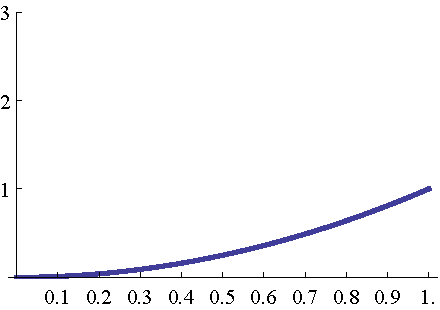
\includegraphics[width=0.45\linewidth]{f} & \quad & 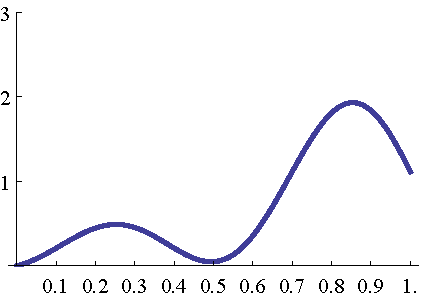
\includegraphics[width=0.45\linewidth]{g}
	\end{array} \] 
\end{myexc}

\begin{theorem}
	For any points \bd{P} and \bd{Q} in linear space $\mathbb{L}$, there is a unique point \bd{Y} such that $\bd{P}+\bd{Y} = \bd{Q}$.
\end{theorem}
\vspace{-.3in}\hspace{5in}\begin{annotation}
	\endnote{Again, remind the students that they have proved this before in the special case $\mathbb{L} = \mathbb{R}^3$  but that now they must use the definition of linear space and not assume points are triples of real numbers. Students who struggled with the last proof often gain confidence after proving this one.}
\end{annotation}


\begin{defn}
		Let \bd{P} and \bd{Q} be points in linear space $\mathbb{L}$. The \bd{difference of \bd{Q} from \bd{P}} is the point, written $\bd{Q}-\bd{P}$, that when added to \bd{P} results in \bd{Q}. In symbols: $\bd{Q}-\bd{P}$ is the vector such that $\bd{P} + (\bd{Q}-\bd{P}) = \bd{Q}$.
\end{defn}

\section{Distributing over a Difference }    \label{Distributing over a Difference}

\begin{defn}
	The \bd{set of all polynomials} is $\mathbb{P}= \{ c_0+c_1x+c_2x^2+\cdots+c_kx^k | \; c_i \in \mathbb{R}, k \in \mathbb{Z}^+ \}$. The \bd{set of polynomials of degree less than n} is $\mathbb{P}_n = \{ c_0+c_1x+c_2x^2+\cdots+c_kx^k | \; c_i \in \mathbb{R}, k \in \mathbb{Z}^+, k<n \}$. In both cases addition and scalar multiplication are done in the traditional way. 
\end{defn}

\begin{myexa}[\bd{a}]
	 Is $\mathbb{P}$ a linear space?
\end{myexa}


\begin{myexb}[\bd{b}]
	Is the set of polynomials of degree exactly 3 a linear space? Is the set of polynomials of degree less than 3 a linear space?  Why is $\mathbb{P}_n$ defined the way it is?
\end{myexb}

\begin{myexc}[\bd{c}]
	Write Theorem 8 as a sentence in English.
\end{myexc}

\begin{theorem}
	For any points \bd{P} and \bd{Q} in linear space $\mathbb{L}$, and any  $c\in\mathbb{R}$:
	\[c(\bd{Q}-\bd{P})=c\bd{Q}-c\bd{P}\]
	\\
\end{theorem}
\vspace{-.3in}\hspace{5in}\begin{annotation}
	\endnote{This theorem is an exercise in careful use of the axioms and previous two theorems.}
\end{annotation}

\noindent \bd{Challenge 8.}  Is \bd{0}, the additive identity element in a linear space, unique?

\section{When the Scalar Multiple is 1}    \label{When the Scalar Multiple is 1}

\begin{myexa}[\bd{a}]
	What is the notation for the additive inverse of $-\bd{Q}$? Find a vector other than $\bd{Q}$ which satisfies the definition of additive inverse for~$-\bd{Q}$.
\end{myexa}

\begin{myexb}[\bd{b}]
   Show: $-(-\bd{Q})=1\bd{Q}$.
\end{myexb}

\begin{myexc}[\bd{c}]
	Can a linear space have exactly one element?  Include justification. 
\end{myexc}

\begin{theorem}
	For any point \bd{P} in linear space $\mathbb{L}$:
	\[1\bd{P} = \bd{P} \]
\end{theorem}
\vspace{-.3in}\hspace{5in}\begin{annotation}
	\endnote{This theorem can be proven in two very different ways. The more subtle way is hinted at in the excercises and relys on the uniquenss of the inverse of $-\bd{P}$.  The other way uses that $\bd{P} +-1\bd{P} = \bd{0}$ from theorem 6 and that $0\bd{P} =\bd{0}$ from Axiom 4.  }
\end{annotation}


\noindent \bd{Challenge 9.} Can a linear space have exactly two elements?

\section{Subspaces }    \label{Subspaces}

\begin{defn} 
	A subset $\mathbb{M}$ of a linear space $\mathbb{L}$ is a \bd{subspace} of $\mathbb{L}$ if $\mathbb{M}$ is itself a linear space.  This means:\\
     
	 \indent  $\mathbb{M}\subseteq \mathbb{L}$  \\
	 
	  $\bullet$ $\mathbb{M}$ is closed under addition: \bd{P}, \bd{Q} $\in \mathbb{M} \Rightarrow \bd{P} + \bd{Q} \in \mathbb{M} $ 
	 
	  $\bullet$ $\mathbb{M}$ is closed under scalar multiplication: $c \in \mathbb{R}$, \bd{P} $\in \mathbb{M} \Rightarrow $ c$\bd{P} \in \mathbb{M}$ \\
	  
	 $\mathbb{M}$ satisfies Axioms $1- 7$ for linear spaces\\

\end{defn}

\begin{myexa}[\bd{a}]
   Is $\mathbb{R}^3 \subseteq \mathbb{R}^3$? \quad Is $\{\} \subseteq \mathbb{P}$? \quad Is $\mathbb{R}^2 \subseteq \mathbb{R}^3$? \quad Is $\mathbb{P} \subseteq$ C[0,1]?
\end{myexa}

\begin{myexb}[\bd{b}]
	Write out several elements in the sets described using set notation below:
		\begin{tabbing}
			\indent i. \quad  \= $\mathbb{S}=\{ x \; |\; 3x \in \mathbb{Z} \}$\\
			\indent ii. \> \= $\mathbb{S}=\{ 3x \; |\; x \in \mathbb{Z} \}$\\
		\end{tabbing}
\end{myexb}

\begin{myexc}[\bd{c}]
	Which of the following sets $\mathbb{M}$ are subspaces of the given linear space? If a set is not a subspace which properties of subspace does it fail to satisfy? 
	\begin{tabbing}
		\indent i. \quad  \= $\mathbb{M}=\{ \ot{x}{y}{0} \; |\; x,y \in \mathbb{R} \}\subseteq \mathbb{R}^3$\\
		\indent ii.\> \= $\mathbb{M}=\{ \ot{x}{y}{z} \;|\; z=x+y,\;x,y\in \mathbb{R}\}=\{\ot{x}{y}{x+y}\;|\;  x,y \in \mathbb{R}\}\subseteq \mathbb{R}^3$\\
		\indent iii. \> \= $\mathbb{M}=\{ \ot{x}{y}{z} \; |\; x,y,z \in \mathbb{R}^+ \}\subseteq \mathbb{R}^3$\\
		\indent iv. \> \= $\mathbb{M}=\{ c_0+c_1x+c_2x^2\; |\; c_i\in \mathbb{Z} \}\subseteq \mathbb{P}$\\
		\indent v. \> \= $\mathbb{M}=\{ f(x)\in C[0,1]\; |\; f(0) = \frac{1}{4} \}\subseteq C[0,1]$\\
		\indent vi. \> \= $\mathbb{M}=\{ f(x)\in C[0,1]\; |\; f(\frac{1}{4}) = 0 \}\subseteq C[0,1]$\\
		\indent vii. \> \= $\mathbb{M}=\{ f(x)\in C[0,1]\; |\; f\ '(x) \in C[0,1] \}\subseteq C[0,1]$\\
	\end{tabbing}
\end{myexc}

\begin{theorem}
	Given a non-empty subset $\mathbb{M}$ of a linear space $\mathbb{L}$. $\mathbb{M}$ is a subspace of  $\mathbb{L}$ if and only if  $\mathbb{M}$ is closed under both addition and multiplication.
\end{theorem}
\vspace{-.3in}\hspace{5in}\begin{annotation}
	\endnote{This is the first of many ``if and only if'' proofs. I encourage students to have a plan for proving such statments that makes it very clear at each point what they are assuming and what they are needing to show. In particlar their proof should have two clearly separate parts.  In one of these parts the students begin by thinking they have to show each of the seven axioms hold.  As they write out their reasoning for each one I encourage them to try to generalize their argument. ( Something along the lines of ``If the axiom is true for all points in $\mathbb{L}$ then it will be true for all points in a subset set of $\mathbb{L}$'', or ``Let \bd{P},\bd{Q} and \bd{R} be points in the subset $\mathbb{M}$, then they are points in  $\mathbb{L}$  and so Axioms 1,2,4,5,6 and 7 hold.'' Students who really get it will identify that Axiom 3, which deals with existence, must be dealt with differently.)}
\end{annotation}
 

\noindent \bd{Challenge 10.} A non-empty subset $\mathbb{M}$ of a linear space $\mathbb{L}$ is a subspace of $\mathbb{L}$ if and only if for any \bd{P} and \bd{Q} in $\mathbb{M}$ and every pair of real numbers $a$ and $b$, $a\bd{P}+b\bd{Q} \in \mathbb{M}$.

\section{Span}    \label{Span}
     
\begin{defn}
	A point \bd{P} is said to be a \bd{linear combination of the points}: $ \bd{P}_1 , \bd{P}_2,\ldots,\bd{P}_n$ if $\bd{P} = t_1\bd{P}_1+ t_2\bd{P}_2+ \cdots+ t_n\bd{P}_n $ for some list of real numbers $t_i$.
\end{defn}

\begin{defn}
	The set of all linear combinations using points from a non-empty set\\ $\mathbb{S}=\{ \bd{P}_1, \bd{P}_2, \ldots, \bd{P}_n \}$ is called the \bd{span} of $\mathbb{S}$, and written: \[span\mathbb{S} = \{\ t_1\bd{P}_1+t_2\bd{P}_2+\cdots+t_n\bd{P}_n\ | \; t_i  \in \mathbb{R}\ \} \]
\end{defn}

\begin{defn}
	A set $\mathbb{S}$ of points in $\mathbb{L}$ is said to \bd{span} $\mathbb{L}$ if $span\mathbb{S}=\mathbb{L}$. This means that every point in $\mathbb{L}$ is a linear combination of the points in $\mathbb{S}$. (Note: Span has again been defined as a noun and as a verb.)
\end{defn}

\begin{myexa}[\bd{a}]
	 Describe the span of $\mathbb{S} = \{ \ot{1}{0}{1},\ot{0}{1}{1}\}$. Does $\mathbb{S}$ span $\mathbb{R}^3$?
\end{myexa}

\begin{myexb}[\bd{b}]
	 Does $\mathbb{S} = \{ x,x^2\}$ span $\mathbb{P}_3$?  If not, find a set that does. 
\end{myexb}

\begin{myexc}[\bd{c}]
	Find two different sets that span $\mathbb{R}^3$?
\end{myexc}

\begin{theorem}
	If  $\mathbb{S}$ is a nonempty subset of a linear space $\mathbb{L}$, then $span\mathbb{S}$ is a subspace of $\mathbb{L}$.  Moreover, $span\mathbb{S}$ is the smallest subspace of $\mathbb{L}$ containing $\mathbb{S}$, in other words, any subspace of $\mathbb{L}$ containing $\mathbb{S}$ must also contain $span\mathbb{S}$.
\end{theorem}
\vspace{-.3in}\hspace{5in}\begin{annotation}
	\endnote{This is a good opportunity for student to use Theorem 10, but if they dont realize this themselves I let them check all the criteria for subspace which gives them a better understanding of Theorem 10. }
\end{annotation}


\noindent \bd{Discussion Question 11.} What definition for $span\{\}$ would make Theorem 11 true without the condition that $\mathbb{S}$ be non-empty?

\section{Linear Independence}    \label{Linear Independence}

\begin{defn}
	 A subset $\mathbb{S} = \{ \bd{P}_1,\bd{P}_2,\ldots,\bd{P}_n\}$  of a linear space $\mathbb{L}$ is \bd{linearly independent} if every point \bd{Q} in $span\mathbb{S}$ can be written in only one way as a linear combination using elements of $\mathbb{S}$. More specifically, for any real numbers $a_1,a_2,\ldots,a_n$  and $b_1,b_2,\ldots,b_n$: 
	 	\[ a_1\bd{P}_1 + a_2\bd{P}_2 +\cdots+a_n\bd{P}_n = b_1\bd{P}_1 + b_2\bd{P}_2 +\cdots+ b_n\bd{P}_n  \Longrightarrow a_1=b_1,\ldots a_n=b_n \]
	 A subset $\mathbb{S}$ is \bd{linearly dependent}  if $\mathbb{S}$ is not linearly independent. 
\end{defn}
   
\begin{myexa}[\bd{a}]
	Show how to write the point $\ot{a}{b}{c}$ as a linear combination of the points in $\mathbb{S} = \{ \ot{1}{2}{0},\ot{1}{0}{0},\ot{1}{1}{0} \}$. Is the set $\mathbb{S}$ linearly independent? If it is not, show how some point can be written in more than one way as a linear combination of the elements of $\mathbb{S}$.
\end{myexa}

\begin{myexb}[\bd{b}]
	What is the additive identity element in the linear space~$\mathbb{R}^n$? \quad ...in the linear space $\mathbb{P}$? \quad ..in the linear space C[0,1]?
\end{myexb}

\begin{myexc}[\bd{c}]
	Describe the steps needed to prove:\[ (A \Longrightarrow B) \Longleftrightarrow (C \Longrightarrow D)\]
\end{myexc}

\begin{theorem}
	Let $\mathbb{S} = \{ \bd{P}_1 , \bd{P}_2 ,\ldots, \bd{P}_n \}$ be a subset of  linear space $\mathbb{L}$. Then the set  $\mathbb{S}$ is linearly independent if and only if for all real numbers $c_1,c_2,\ldots,c_n$, $c_1\bd{P}_1 + c_2\bd{P}_2 +\cdots+c_n\bd{P}_n = \bd{0}$  implies all of the coefficients $c_i$ are zero.
\end{theorem}
\vspace{-.3in}\hspace{5in}\begin{annotation}
	\endnote{The most difficult part of this proof is setting it up correctly. It is also important that student are clear that $A \Rightarrow B$ being true does not mean $A$ must be true.  }
\end{annotation}

\section{When a Set Contains 0}    \label{When a Set Contains 0}

\begin{myexa}[\bd{a}]
	Negate the following:
		\begin{tabbing}
			\indent i. \quad  \= It is raining $\Longrightarrow$ there are clouds in the sky\\
			\indent ii.\> For any math problem there is a solution. \\
			\indent iii. \> For all integers, prime $\Longrightarrow$ odd\\
			\indent iv. \> $x=1, \; y=2$, and $z=3$\\
		\end{tabbing}
\end{myexa}

\noindent \bd{Discussion Question 13.} Do the following mean the same thing?\\
\indent ``For any \ldots'' \quad  ``For all\ldots'' \quad ``For every\ldots''

\begin{myexb}[\bd{b}]
	Negate the definition of $\mathbb{S}$ being linearly independent to get a definition for $\mathbb{S}$ being linearly dependent.
\end{myexb}

\begin{myexc}[\bd{c}]
	Show how to write the point $\ot{a}{b}{c}$ as a linear combination of the points in $\mathbb{S} = \{  \ot{1}{2}{0}, \ot{1}{0}{0}, \ot{1}{1}{1}  \}$. Is the set  $\mathbb{S}$ linearly independent?
\end{myexc}

\begin{theorem} 
	If $\mathbb{S}$ is a subset of a linear space $\mathbb{L}$ and \bd{0} $\in \mathbb{S}$, then $\mathbb{S}$ is linearly dependent.
\end{theorem}
\vspace{-.3in}\hspace{5in}\begin{annotation}
	\endnote{This is a very short proof and I find it best not to give the students too much help except perhaps to help them identify that this is a proof of existence and as such the more specific they can be the better.  }
\end{annotation}

\section{Linear Dependence}    \label{Linear Dependence}

\begin{myexa}[\bd{a}]
	Is the set $\mathbb{S} = \{x^2-1,\  x+1,\  x-1 \} $  linearly independent in $\mathbb{P}_3$?
\end{myexa}

\begin{myexb}[\bd{b}]
	Is the set $\mathbb{S} = \{1,\  sin^2(x),\  cos^2(x) \} $ linearly independent in C[0,1]?
\end{myexb}

\begin{myexc}[\bd{c}]
	Use Theorem 12 to write another condition for $\mathbb{S}$ to be linearly dependent. 
\end{myexc}

\begin{theorem}
	Let $\mathbb{S}$ be a subset of a linear space $\mathbb{L}$ containing more than one point. $\mathbb{S}$ is linearly dependent if and only if some point of $\mathbb{S}$ is a linear combination of the other points of $\mathbb{S}$. 
\end{theorem}
\vspace{-.3in}\hspace{5in}\begin{annotation}
	\endnote{  I often arrange for weakers students to be in the same group for this theorem since here they can demonstrate mastery of proving ``if and only if'' statements and the definition of linearly dependent. }
\end{annotation}


\noindent \bd{Discussion Question 14.}
   The definition, Theorem 12, and Theorem 14 give three equivalent criteria for a set to be linearly independent. Which matches the meaning of ``independent'' most closely? Which seems easiest to use to prove set is linearly independent? Which makes the most sense paired with the definition of span? What do traditional Linear Algebra texts have for the definition of linearly independent? 
   
\section{Extending Linearly Independent Sets}    \label{Extending Linearly Independent Sets}   

\begin{myexa}[\bd{a}]
	Describe how to show a set $\mathbb{S}$ spans a linear space $\mathbb{L}$. Describe 3 ways to show a set $\mathbb{S}$ is linearly independent. 
\end{myexa}

\begin{myexb}[\bd{b}]
	Show $\{ \oq{1}{1}{0}{0},\oq{0}{1}{1}{0},\oq{0}{0}{1}{1} \} $ is linear independent in $\mathbb{R}^4$. Does is also span $\mathbb{R}^4$?
\end{myexb}

\begin{myexc}[\bd{c}]
	Given that $\mathbb{S} = \{ \ot{1}{0}{0},\ot{0}{1}{0} \} $ is linearly independent in $\mathbb{R}^3$, find a point \bd{P} such that $\mathbb{S} \cup \{\bd{P}\}$ is also linearly independent. Describe all possible such points. 
\end{myexc}

\begin{theorem}
	If $\mathbb{S}$ is a linearly independent subset of $\mathbb{L}$ and \bd{P} is a point of $\mathbb{L}$, not in $span(\mathbb{S})$, then $\mathbb{S} \cup \{ \bd{P} \}$ is also linearly independent. 
\end{theorem}
\vspace{-.3in}\hspace{5in}\begin{annotation}
	\endnote{For this theorem students can use any of the three equivalent criteria for linear independence. You may have to point out that just not being able to write the new point as a linear combination of the old points is not good enough, they would also have to show that no old point can be written as a linear combination of union of the new point and the other old points.   }
\end{annotation}


\begin{defn}
	A finite subset $\mathbb{B}$ of a linear space $\mathbb{L}$ is a \bd{basis} if each point in $\mathbb{L}$ can be written in one and only one way as a linear combination of elements of $\mathbb{B}$. In other words, $\mathbb{B}$ is a basis for $\mathbb{L}$ if it spans $\mathbb{L}$ and is linearly independent.
\end{defn}

\noindent \bd{Discussion Question 15.} For infinite subsets $\mathbb{B}$ of $\mathbb{L}$  define $span(\mathbb{B})$ to be the set of all linear combinations involving a finite number of element of $\mathbb{B}$. With this addition the definitions of span and linearly independent can be extended to infinite subsets of $\mathbb{L}$. Thus a basis may contain an infinite number of elements; however, only a finite number of them may be used when making linear combinations. What problems could occur if infinite sums were allowed for linear combinations? 

\section{Maximal Linearly Independent Sets}    \label{Maximal Linearly Independent Sets}

\begin{myexa}[\bd{a}]
	Is $\mathbb{S} = \{ \ot{1}{2}{3},\ot{1}{2}{0},\ot{1}{0}{0} \} $ a basis for $\mathbb{R}^3$?  Explain.
\end{myexa}

\begin{myexb}[\bd{b}]
	Is $\mathbb{S} = \{x^2+1, x+1, x-1 \} $ a basis for $\mathbb{P}_3$? Explain.
\end{myexb}

\begin{myexc}[\bd{c}]
	State Theorem 15 in words.
\end{myexc}

\begin{theorem}
	$\mathbb{S}$ is a basis for $\mathbb{L}$ if and only if it is a maximal linearly independent subset of $\mathbb{L}$. In other words, $\mathbb{S}$ is a basis for $\mathbb{L}$ if and only if $\mathbb{S}$ is linearly independent and not a proper subset of any other linearly independent set. 
\end{theorem}
\vspace{-.3in}\hspace{5in}\begin{annotation}
	\endnote{You may need to talk about the concept of maximal which is not the same as biggest. }
\end{annotation}


\section{Reducing a Spanning Set}    \label{Reducing a Spanning Set}

\begin{myexa}[\bd{a}]
	Show how to write the point $\bd{A} = \ot{a}{b}{c}$  as a linear combination of the points in $\mathbb{S} = \{ \ot{1}{0}{-1},\ot{1}{2}{3},\ot{3}{2}{1},\ot{0}{1}{0} \} $. Are all the points in $\mathbb{S}$ necessary?
\end{myexa}

\begin{myexb}[\bd{b}]
	Find a subset of $\mathbb{S} = \{ \ot{1}{0}{-1},\ot{1}{2}{3},\ot{3}{2}{1},\ot{0}{1}{0} \} $  that spans $\mathbb{R}^3$.
\end{myexb}

\begin{myexc}[\bd{c}]
	Find a subset of $\mathbb{S} = \{ \ot{1}{0}{-1},\ot{1}{2}{3},\ot{3}{2}{1},\ot{0}{1}{0} \} $  that does not span $\mathbb{R}^3$.
\end{myexc}

\begin{theorem}
	If  $\mathbb{S}$ spans $\mathbb{L}$ and \bd{P} is a point of $\mathbb{S}$ such that \bd{P} $\in span(\mathbb{S}-\{\bd{P}\})$ then  $\mathbb{S}-\{\bd{P}\}$ also spans $\mathbb{L}$. 
\end{theorem}
\vspace{-.3in}\hspace{5in}\begin{annotation}
	\endnote{Here is a good proof to get students used to identifying what they are being asked to prove, and in this case identify what a proof that a set spans $\mathbb{L}$ should look like.  }
\end{annotation}

\section{Minimal Spanning Sets}    \label{Minimal Spanning Sets}

\begin{myexa}[\bd{a}]
	Find a basis for $\mathbb{R}^n$. Now find a different basis for $\mathbb{R}^n$.
\end{myexa}

\begin{myexb}[\bd{b}]
	Find two different bases for $\mathbb{P}_n$.  Find a basis for $\mathbb{P}$.
\end{myexb}

\begin{myexc}[\bd{c}]
	State theorem 17 in words.
\end{myexc}

\begin{theorem}
	$\mathbb{S}$ is a basis for $\mathbb{L}$ if and only if $\mathbb{S}$ is a minimal spanning set for $\mathbb{L}$. In other words $\mathbb{S}$ is a basis for $\mathbb{L}$ if and only if $\mathbb{S}$ spans $\mathbb{L}$ and no proper subset of $\mathbb{S}$ spans $\mathbb{L}$.
\end{theorem}
\vspace{-.3in}\hspace{5in}\begin{annotation}
	\endnote{This theorem is similar to Theorem 16. }
\end{annotation}

\section{The Replacement Lemma}    \label{The Replacement Lemma}

\begin{myexa}[\bd{a}]
      Is the set $\{1, x, x^2, x^3, \ldots,x^n, \ldots\}$ a basis for C[0,1]?	
 \end{myexa}

\begin{myexb}[\bd{b}]
	Consider the set $\mathbb{S}=\{\ot{1}{0}{1}, \ot{0}{1}{0} \}$ which spans some subspace $\mathbb{L} \subseteq \mathbb{R}^3$. Notice \ot{2}{3}{2} is a linear combination of the points in $\mathbb{S}$ since $\ot{2}{3}{2} =2\ot{1}{0}{1}+ 3\ot{0}{1}{0}$. Consider the set $\mathbb{S}' = \{ \ot{1}{0}{1}, \ot{2}{3}{2} \}$. Show how the point \ot{0}{1}{0} can be written as a linear combination of the points in $\mathbb{S}'$? Does $\mathbb{S}'$ also span $\mathbb{L}$? Explain.
\end{myexb}

\begin{myexc}[\bd{c}]
	If  $\bd{Q} = 2\bd{P}_1+3\bd{P}_2 + 0\bd{P}_3 + 4\bd{P}_4 + -1\bd{P}_5 + 0\bd{P}_6$ which \bd{P}'s can be written as linear combinations \bd{Q} and the other \bd{P}'s?
\end{myexc}

\begin{theorem}[Replacement Lemma]
	Suppose that $\mathbb{S}$  spans $\mathbb{L}$, $\bd{Q} \in \mathbb{L}$ and \bd{P} is a point of $\mathbb{S}$ such that when \bd{Q} is written as a linear combination of points of $\mathbb{S}$, the coefficient of \bd{P} is not zero. If $\mathbb{S}'$ is the set obtained from $\mathbb{S}$ by replacing \bd{P} with \bd{Q}, then $\mathbb{S}'$ also spans $\mathbb{L}$. 
\end{theorem}
\vspace{-.3in}\hspace{5in}\begin{annotation}
	\endnote{This theorem is really a lemma and a good opportunity to point out the purpose of lemmas so that students can watch for where this lemma can be used.   }
\end{annotation}

\section{Preparing to Define Dimension} \label{Preparing to Define Dimension}


\noindent \bd{Discussion Question 20.}
What problems might occur if the Dimension of a Vector Space were defined to be the number of elements in a basis? How is this similar to other situations where the term 'well defined'  is used?

\begin{myexa}[\bd{a}]
	Does Theorem 16 say there is no linearly independent set with more elements than a basis?  Explain. 
\end{myexa}

\begin{myexb}[\bd{b}]
	Does Theorem 18 say there is no spanning set with fewer elements than a basis? 
\end{myexb}

\begin{myexc}[\bd{c}]
	Find another way to state Theorem 20.
\end{myexc}

\begin{theorem}
	Considering only finite subsets of $\mathbb{L}$, no linearly independent set has more points than a spanning set.
\end{theorem}
\vspace{-.3in}\hspace{5in}\begin{annotation}
	\endnote{This may be the hardest theorem in these notes. I usually give the hint that if one set is a subset of another set it can't have more points than that set. This proof should start with taking an arbitrary linearly independent set and an arbitrary spanning set. The replacement lemma can then be used to define a sequence of spanning sets that element by element take in every element of the linearly independent set.  Pictures are helpful. For weaker students I suggest they start by assuming the linearly independent set has only three elements. Otherwise I suggest writing out at least three iterations and then generalizing. }
\end{annotation}

\section{Properties of Linearly Independent Sets}    \label{Properties of Linearly Independent Sets}


\begin{myexa}[\bd{a}]
	Is there an infinite subset in C[0,1] which is linearly independent? To demonstrate such a set one option is to use pictures and establish a pattern.
\end{myexa}

\begin{myexb}[\bd{b}]
	Describe how to extend a linearly independent set to get a basis. Will this always work?
\end{myexb}

\begin{myexc}[\bd{c}]
	Use negation to rewrite Theorem 16. 
\end{myexc}

\begin{theorem}
	If $\mathbb{L}$ has a basis $\mathbb{B} = \{ \bd{P}_1, \bd{P}_2,\ldots,\bd{P}_n \}$ with a finite number of points, then the following hold:
	\begin{tabbing}
		\indent i. \quad  \= No linearly independent set contains more than $n$ points.\\
		\indent ii.\> Every linearly independent set with $n$ points is a basis.\\ 
		\indent iii. \> Every linearly independent set is contained in a basis.
	\end{tabbing}
\end{theorem}
\vspace{-.3in}\hspace{5in}\begin{annotation}
	\endnote{ Here the hard work of the previous theorems pay off.  }
\end{annotation}

\section{Properties of Spanning Sets}    \label{Properties ofSpanning Sets}

\begin{myexa}[\bd{a}]
	Show that no finite set spans C[0,1].
\end{myexa}

\begin{myexb}[\bd{b}]
	Describe how to reduce a spanning set to get a basis. Will this always work?
\end{myexb}

\begin{myexc}[\bd{c}]
	Use negation to rewrite Theorem 18.
\end{myexc}

\begin{theorem}
    If $\mathbb{L}$ has a basis $\mathbb{B} = \{ \bd{P}_1, \bd{P}_2,\ldots,\bd{P}_n \}$ with a finite number of points, then the following hold:
    \begin{tabbing}
    	\indent i. \quad  \= No spanning set contains fewer than $n$ points.\\
    	\indent ii.\> Every spanning set with $n$ points is a basis.\\ 
    	\indent iii. \> Every finite spanning set containes a basis.
    \end{tabbing}
\end{theorem}
\vspace{-.3in}\hspace{5in}\begin{annotation}
	\endnote{ Student may need help identifing  why the condition of ``finite''  is given in part \it{iii.}  }
\end{annotation}
\\

Theorems 21 and 22 together give the result that if a linear space has a basis with $n$ points, then every basis must have $n$ points. This observation leads to the following important definition. 


\begin{defn}
	If a linear space $\mathbb{L}$ has a basis with $n$ elements  $\mathbb{L}$ is called an \bd{n dimensional vector space}. If there is no finite set that forms a basis for $\mathbb{L}$,  $\mathbb{L}$ is said to be \bd{infinite dimensional}.
\end{defn}

\section{When the Vectors are the Rows}    \label{When the vectors are the Rows}

Until now our ordered n-tuples have appeared in matrices as columns.  They can also be placed as rows. The following Theorem shows what can be learned by row-reducing such a matrix. 

\begin{myexa}[\bd{a}]
	Put the points of $\mathbb{S} = \{ \ot{3}{0}{-3}, \ot{1}{2}{3}  \}$ into a matrix as rows then row reduce the resulting matrix. Use $\mathbb{S}'$ to denote the rows of the resulting matrix. What does Theorem 23 say about $span\mathbb{S}'$?
\end{myexa}

\begin{myexb}[\bd{b}]
	Find a ``nicer'' set that spas the same space as the set spanned by $\mathbb{S} = \{ \ot{3}{0}{-3}, \ot{1}{2}{3},\ot{0}{1}{0}  \}$. Is this new set linearly independent?
\end{myexb}

\begin{myexc}[\bd{c}]
    Find a ``nicer'' set that spans the same space as the set spanned by $\mathbb{S} = \{ \ot{3}{0}{-3}, \ot{1}{2}{3}, \ot{3}{2}{1} ,\ot{0}{1}{0}  \}$. Is this new set linearly independent?
\end{myexc}

\begin{theorem}
	Let $\mathbb{S}$ be a subset of a linear space $\mathbb{R}^n$ and let \bd{P} be in $\mathbb{S}$. Assume that \bd{Q} is obtained from \bd{P} either by 
	 \begin{tabbing}
	 	\indent i. \quad  \= multiplying \bd{P} by a non-zero number \quad  \bd{or}\\
	 	\indent ii.\>adding to \bd{P} a scalar multiple of another element of $\mathbb{S}$ 
	 	 \end{tabbing}
	Let $\mathbb{S}'$ be obtained from $\mathbb{S}$ by replacing \bd{P} with \bd{Q}. Then $\mathbb{S}'$ will span the same linear space as $\mathbb{S}$. In other words: $span\mathbb{S}' = span\mathbb{S}$.\\ \\
	In addition, if $\mathbb{S}''$ consists of the non-zero rows of a fully simplified matrix, then $\mathbb{S}''$ is linearly independent.
\end{theorem}
\vspace{-.3in}\hspace{5in}\begin{annotation}
	\endnote{ The first half of this theorem is another application of the Replacement Lemma.  For the second half, that every nonzero row has a leading 1 in a position in which all the other rows will have zeros, is the key to showing the nonzero rows are linearly independent. }
\end{annotation}



% \iffalse  % to omit ch 3

%%%%%%%%%%%%%%%%%%%%%%%%%%%%%%%%%%%%%%%%%%%%%%%%%%%%%%%%%%%%%%%%%%%%%%%%%%%%%%%%%%%%%%%
%%%%%%%%%%%%%%%%%%%%%%%%%%%%%%%%%%%%%%%%%%%%%%%%%%%%%%%%%%%%%%%%%%%%%%%%%%%%%%%%%%%%%%%
%%%%%%%%%%%%%%%%%%%%%%%%%%%%%%%%%%%%%%%%%%%%%%%%%%%%%%%%%%%%%%%%%%%%%%%%%%%%%%%%%%%%%%%

\chapter{Linear Transformations}    \label{Linear Transformations}
Functions play a central role in mathematics and linear combinations play a central role in Linear Algebra. We want a type of function that respects the organization of points into linear combinations. Throughout $\mathbb{L}_1, \mathbb{L}_2$ and $\mathbb{L}_3$ will be general linear spaces.

\section{Properties of Linear Transformations}    \label{Properties of Linear Transformations}

\begin{defn} A \bd{linear transformation} is a function $f: \mathbb{L}_1 \longrightarrow \mathbb{L}_2$, such that for any \bd{P}, \bd{Q} $\in \mathbb{L}_1$, and $c \in \mathbb{R}$: 
	\begin{tabbing}
		\indent 1. \quad \= $f(\bd{P}+\bd{Q}) = f(\bd{P})+f(\bd{Q}) $\\
		\indent 2. \> $f(c\bd{P}) = cf(\bd{P})$ 
	\end{tabbing}
\end{defn}


\begin{myexa}[\bd{a}]
	If $T:\mathbb{L}_1 \longrightarrow \mathbb{L}_2$ is a linear transformation explain why:
	\begin{tabbing}
		\indent i. \quad \= $T(\bd{0}) = \bd{0}$ \\
		\indent ii. \> $T( -\bd{A}) = -T(\bd{A})$ for any \bd{A} $\in \mathbb{L}_1$\\
		\indent iii. \> $T(\bd{A}-\bd{B}) = T(\bd{A})-T(\bd{B})$ for any \bd{A}, \bd{B} $\in \mathbb{L}_1$\\
	\end{tabbing}
\end{myexa}

\begin{myexb}[\bd{b}]
	Which of the following are functions?
	\begin{tabbing}
		\indent i. \quad \= $f:\mathbb{Q}$ \ \=$\rightarrow \mathbb{Q} $\ \ \   \=defined by $f(\frac{a}{b})= ab$   \\
		\indent ii. \> $g:\mathbb{Q}$ \>$\rightarrow \mathbb{Q} $ \>defined by  $g(\frac{a}{b}) = \frac{b}{a}$ \\ 
		\indent iii. \> $h:\mathbb{Q}^2 $ \>$\rightarrow \mathbb{Q} $ \>defined by  $h(\frac{a}{b},\frac{c}{d}) = \frac{ac}{bd}$  \\
		\indent iv. \>  $j:\mathbb{Q} $ \>$\rightarrow \mathbb{Q}^2 $ \>defined by  $j(\frac{a}{b}) = (a,b)$  \\  
		\indent v. \>  $k:\mathbb{Q} $ \>$\rightarrow \mathbb{Q} $ \>defined by  $k(\frac{a}{b}) = \frac{a^2}{b^2}$  
	\end{tabbing}
	Which of the following functions are linear transformations?
	\begin{tabbing}
		\indent i. \quad \= $f:\mathbb{R}$ \ \=$\rightarrow \mathbb{R} $\ \ \   \=defined by $f(x)= x^2$   \\
		\indent ii. \> $g:\mathbb{R}$ \>$\rightarrow \mathbb{R} $ \>defined by  $g(x) = 3x+1$ \\ 
		\indent iii. \> $h:\mathbb{R}^3 $ \>$\rightarrow \mathbb{R}^2 $ \>defined by  $h(x_1,x_2,x_3) = (x_1,x_2)$  \\
		\indent iv. \>  $j:\mathbb{P} $ \>$\rightarrow \mathbb{R}$ \>defined by  $k(p(x)) = p(1)$ \\
		\indent v. \>  $k:C[0,1] $ $\rightarrow C[0,1] $ defined by  $k(x) = k\ '(x)$      
	\end{tabbing} 
	Which of the following functions are $1-1$? 
	\begin{tabbing}
		\indent i. \quad \= $f:\mathbb{R}^2$ \ \=$\rightarrow \mathbb{R}^2 $\ \ \   \=defined by $f(x_1,x_2)= (x_2 ,x_1)$  \\
		\indent ii. \> $g:\mathbb{R}^2$ \>$\rightarrow \mathbb{R}^2 $ \>defined by  $g(x_1, x_2) = (x_1,0) $ \\ 
		\indent iii. \> $h:C[0,1] \rightarrow C[0,1] $ defined by  $h(f) = \int^x_0f $  \\
		\indent iv. \>  $j:C[0,1] \rightarrow \mathbb{R} $ defined by  $h(f) = \int^1_0f $  \\
		\indent v. \>  $k:\mathbb{P} $ \>$\rightarrow \mathbb{P}$ \>defined by  $k(p(x)) = x\cdot p(x)$
	\end{tabbing}
	Which of the following functions are onto?
	\begin{tabbing}
		\indent i. \quad \= $f:\mathbb{R}^2$ \ \=$\rightarrow \mathbb{R}^2 $\ \ \   \=defined by $f(x_1,x_2)= (x_2 ,x_1)$  \\
		\indent ii. \> $g:\mathbb{R}^2$ \>$\rightarrow \mathbb{R}^2 $ \>defined by  $g(x_1, x_2) = (x_1,0) $ \\ 
			\indent iii. \> $h:C[0,1] \rightarrow C[0,1] $ defined by  $h(f) = \int^x_0f $  \\
			\indent iv. \>  $j:C[0,1] \rightarrow \mathbb{R} $ defined by  $h(f) = \int^1_0f $  \\
			\indent v. \>  $k:\mathbb{P} $ \>$\rightarrow \mathbb{P}$ \>defined by  $k(p(x)) = x\cdot p(x)$ 
	\end{tabbing}
\end{myexb}

 \noindent \bd{Discussion Question 24.} For a function to be $1-1$  it must have the property that if you put in two different inputs, $x \neq y$, then their outputs are different, $f(x) \neq f(y)$. Recall that the contrapositive of an implication is equivalent to that implication.  Use the contrapositive to rewrite what it means for a function for be $1-1$.  What does it mean for a function to be onto? 
 
 \vspace{.5cm}
\begin{myexc}[\bd{c}]
Show 
\begin{tabbing}
	\indent i. \quad \= $f:\mathbb{R}^2 \longrightarrow \mathbb{R}^3 $ defined by $f(x_1,x_2)= (x_1,x_1+x_2,x_1-x_2)$  is $1-1$ \\
	\indent ii. \> $g:\mathbb{R}^4 \longrightarrow \mathbb{R}^2 $ defined by  $g(x_1,x_2,x_3,x_4) = (x_1 \cdot x_2, x_3\cdot x_4)$  is onto
\end{tabbing}
\end{myexc}

\vspace{.5cm}

\begin{theorem} Let $\mathbb{L}_1 $,$\mathbb{L}_2$ and $\mathbb{L}_3$ be linear spaces.
			\begin{tabbing} 
			\indent i. \quad  \= If $T:\mathbb{L}_1 \longrightarrow \mathbb{L}_2 $ is a linear transformation that is $1-1$ and maps onto  $\mathbb{L}_2$ \\ \> then the function $T^{-1}:\mathbb{L}_2 \longrightarrow \mathbb{L}_1$ exists and is also a linear transformation. \\ \\
			\indent ii.\> If  $T_1:\mathbb{L}_1 \longrightarrow \mathbb{L}_2 $ and  $T_2:\mathbb{L}_2 \longrightarrow \mathbb{L}_3 $ are $1-1$, onto linear transformations\\ \> then $T_2 \circ T_1$ is a 1-1, onto linear transformation.
			  \\
		\end{tabbing}
\end{theorem}

\vspace{.5cm}

\section{The Kernel}    \label{The Kernel}

\begin{defn}
	Given a linear transformation $T:\mathbb{L}_1 \longrightarrow \mathbb{L}_2 $ the set of points in $\mathbb{L}_1$ that $T$ sends to $\bd{0} \in \mathbb{L}_2$ is called the \bd{kernel} of $T$ and written:  
	\[ker(T)= \{ \bd{P} \in \mathbb{L}_1  \ |\ T(\bd{P}) = \bd{0} \}  \]. 
\end{defn}

\begin{myexa}[\bd{a}]
	Describe the kernel of $T:\mathbb{R}^3 \longrightarrow \mathbb{R}^3$ if T is the linear transformation that 
		\begin{tabbing} 
				\indent i. \quad  \= rotates all points around the z-axis by 90$^\circ$ \\
				\indent ii. \> projects all points perpendicularly onto the xy-plane \\
				\indent iii.  \> projects all points horizontally onto the z-axis\\
				\indent iv.  \> reflects all points across the xy-plane \\
				\indent v.   \> moves all points straight out to twice their distance from origin
		\end{tabbing}  
\end{myexa}

\begin{myexb}[\bd{b}]
		What is the kernel of $T:C[0,1] \longrightarrow C[0,1]$ if $T$ is the linear transformation defined by $T(f) = f'$. 
\end{myexb}

\begin{myexc}[\bd{c}]
	For $T:\mathbb{R}^2 \longrightarrow \mathbb{R}^3$ find $ker(T)$ and $dim(ker(T))$ if T is the linear transformation defined by 
		\begin{tabbing} 
	\indent i. \quad  \= $T(x,y) = (0, 0, 0)$ \\
 	\indent ii. \> $T(x,y) = (0, 0 ,x+y)$ \\
	\indent iii.  \> $T(x,y) = (x,y,0)$ \\
	\indent iv.  \> $T(x,y) = (x, y, x+y)$ 
		\end{tabbing}  
\end{myexc}

\begin{theorem}
	For any linear transformation $T:\mathbb{L}_1 \longrightarrow \mathbb{L}_2 $, $ker(T) = \{\bd{0}\}$ if and only if $T$  is $1-1$. 
\end{theorem}

\vspace{.5cm}

\section{The Range}    \label{The Range}

\begin{defn}
	Given a linear transformation $T:\mathbb{L}_1 \longrightarrow \mathbb{L}_2 $ the set of points in $\mathbb{L}_2$ that are the result of $T$ applied to at least one element of $\mathbb{L}_1$ is called the \bd{range} of $T$ and written:
	\[T(\mathbb{L}_1)= \{ T(\bd{P}) \  |\ \bd{P} \in \mathbb{L}_1  \}  \]. 
\end{defn}

\begin{myexa}[\bd{a}]
	Describe the range of $T:\mathbb{R}^3 \longrightarrow \mathbb{R}^3$ if T is the linear transformation that 
	\begin{tabbing} 
		\indent i. \quad  \= rotates all points around the z-axis by 90$^\circ$ \\
		\indent ii. \> projects all points perpendicularly onto the xy-plane \\
		\indent iii.  \> projects all points horizontally onto the z-axis\\
		\indent iv.  \> reflects all points across the xy-plane \\
		\indent v.   \> moves all points straight out to twice their distance from origin
	\end{tabbing}  
\end{myexa} 

\begin{myexb}[\bd{b}]
		What is the range of $T:\mathbb{P} \longrightarrow \mathbb{P}$ if $T$ is the linear transformation defined by $T(p(x)) = x\cdot p(x)$. 
\end{myexb}

\begin{myexc}[\bd{c}]
For $T:\mathbb{R}^2 \longrightarrow \mathbb{R}^3$ find $T(\mathbb{R}^2)$ and $dim(T(\mathbb{R}^2))$ if T is the linear transformation defined by 
\begin{tabbing} 
	\indent i. \quad  \= $T(x,y) = (0, 0, 0)$ \\
	\indent ii. \> $T(x,y) = (0, 0 ,x+y)$ \\
	\indent iii.  \> $T(x,y) = (x,y,0)$ \\
	\indent iv.  \> $T(x,y) = (x, y, x+y)$ 
\end{tabbing}  
\end{myexc}

\begin{theorem}
	For any linear transformation $T:\mathbb{L}_1 \longrightarrow \mathbb{L}_2 $
	\begin{tabbing} 
		\indent i. \quad  \=the kernel of $T$, $ker(T)$ is a subspace of $\mathbb{L}_1$ \\ 
		\indent ii.\>  the range of $T$, $T(\mathbb{L}_1)$ is a subspace of $\mathbb{L}_2$
	\end{tabbing}
\end{theorem} 

\vspace{.5cm}

\noindent \bd{Challenge 26.} Prove for any linear transformation $T:\mathbb{L}_1 \longrightarrow \mathbb{L}_2 $ where $\mathbb{L}_1$ is a finite dimensional linear space: $dim(ker(T))+dim(T(\mathbb{L}_1)) = dim(\mathbb{L}_1) $

\section{Isomorphisms}    \label{Isomorphisms}

\begin{defn}
	A function $ F:\mathbb{L}_1\longrightarrow \mathbb{L}_2$ is an \bd{Isomorphism} if $F$ is a linear transformation that is $1-1$ and maps onto $\mathbb{L}_2$. 
\end{defn}


\begin{myexa}[\bd{a}]
	 	Given that $T: \mathbb{R}^3 \longrightarrow \mathbb{R}^2$ is a linear transformation such that $T(1,1,0) = (1,2)$, $T(0,0,1)=(0,-1)$ and $T(0,1,0) =(2,0)$. Determine $T(3,3,0)$, $T(1,2,3)$, and $T(x,y,z)$.
\end{myexa}


 \noindent \bd{Discussion Question 27.} Describe the problems that could occur if the set on which the linear transformation is defined is:
 \begin{tabbing}
 	\indent i. \quad \= not a spanning set for $\mathbb{R}^3$ \\
 	\indent ii. \> not linearly independent 
 \end{tabbing}


 \begin{myexb}[\bd{b}]  Use a system of equations to 
 \begin{tabbing}
 	\indent i. \quad \= write (5,4,3) as a linear combination of (1,1,1),(0,1,1) and (0,0,1).  \\
 	\indent ii. \> write $5+4x +3x^2$ as a linear combination of $1+x+x^2$, $x+x^2$ and $x^2$.
 \end{tabbing}
 \end{myexb}
 

\begin{myexc}[\bd{c}]
	Define a linear transformation from $\mathbb{P}_3$ to $\mathbb{R}^3$. Is it 1-1? Is it onto? What is its inverse transformation? 
\end{myexc}


\begin{theorem}
	Any n-dimensional linear space is isomorphic to $\mathbb{R}^{n}$
\end{theorem}

\noindent \bd{Challenge 27.}   Prove any two n-dimensional linear spaces are isomorphic.

\vspace{.5cm}

\section{Matrices}    \label{Matrices}

From now on assume all linear spaces are finite dimensional and a basis, $\beta$, has been chosen. Each point $\bd{P}$ in the linear space can then be uniquely identified using the list of coefficients used to write $\bd{P}$ as a linear combination of the points in $\beta$.  This list is called its coordinate vector and is written  \[  [\bd{P}]_{\beta} = \left[  \begin{array}{c} c_1\\c_2\\ \vdots \\c_n \end{array} \right]\in\mathbb{R}^n \] 



\noindent For example if $\beta=\{1,x,x^2\}$ and $\alpha = \{1+x+x^2,x+x^2,x^2\}$
 \[ [5+4x+3x^2]_{\beta}= \left[  \begin{array}{c} 5\\4\\3\end{array} \right]  \ \ \text{and} \ \ [5+4x+3x^2]_{\alpha}= \left[  \begin{array}{r} 5\\-1\\-1\end{array} \right] \] 

Lists of coordinate vectors can be organized into what are called coordinate matrices. 



\begin{defn}
	A \bd{Matrix} is a rectangular array of numbers, written \[\mtx{A}_{r \times c}= [a_{ij}] =\left[ \begin{array}{cccc}
	a_{11} & a_{12} & \cdots &  a_{1c}  \\
	a_{21} & a_{22} & \cdots &  a_{2c}  \\
	\vdots & \vdots & \ddots & \vdots  \\
	a_{r1} & a_{r2} & \cdots & a_{rc}
	\end{array} \right] \]
\end{defn}
\vspace{.5cm}
\begin{defn}
	For matrices $\mtx{A}_{r \times c} =[a_{ij}]$ and $\mtx{B}_{ m \times n} = [b_{ij}]$ 
	\begin{tabbing}
		\indent i. \quad  \= The \bd{sum} of \mtx{A} and \mtx{B} is possible when $r=m$ and $c=n$ and is defined by\\  \> \indent $\mtx{A}+\mtx{B} = [s_{ij}]$  where $s_{ij}=a_{ij} + b_{ij}$\\
		\indent ii.\> The \bd{scalar product} of $t \in \mathbb{R}$ and \mtx{A} is defined by\\ \> \indent  $t\mtx{A} = [q_{ij}]$  where $q_{ij} = ta_{ij}$ \\
		\indent iii.\> The \bd{product} of \mtx{A} and \mtx{B} is possible when $c=m$ and is defined by\\ \> \indent  $\mtx{AB} = [p_{ij}]$  where $p_{ij} = a_{i1}b_{1j}+a_{i2}b_{2j}+\cdots+a_{in}b_{nj} $
	\end{tabbing}
\end{defn}
\vspace{.5cm}
\begin{myexa}[\bd{a}]
	Perform, if possible, the indicated matrix operations. 
	\[ \begin{array}{ccc}
		A=\left[ \begin{array}{ccc} 1&2&3 \\ 4&5&6\\ 7&8&9 \end{array}\right] & B=\left[ \begin{array}{rrr} -1&0&1 \\ 1&-1&0\\ 0&0&0 \end{array}\right] & C=\left[ \begin{array}{ccc} 1&10&100 \\ 0&-1&0 \end{array}\right]
	\end{array} \]
	 \begin{tabbing}
	 	\indent i. \quad  \= $3A=$ \hspace{2 in} \= v. \quad \= $3+A =$\\
	 	\indent ii.\>$A+B =$ \> vi. \> $A+C =$ \\
	 	\indent iii. \> $AB =$ \> vii. \> $BA =$  \\
	 	\indent iv. \> $AC =$ \> viii. \> $CA =$ 
	 \end{tabbing}
\end{myexa}

\begin{defn}
	An \bd{additive identity} for the set of $n \times n$ matrices is an $n \times n$ matrix \mtx{O} such that for all $n \times n$ matrices \mtx{M}, $\mtx{M}+\mtx{O} = \mtx{M}$.  \mtx{O} is also called the zero matrix. A \bd{multiplicative identity} for the set of $n \times n$ matrices is an $n \times n$ matrix \mtx{I} such that for all $n \times n$ matrices \mtx{M}, $\mtx{MI} = \mtx{M}$  and $\mtx{IM} = \mtx{M}$. 
\end{defn}

\begin{myexb}[\bd{b}]
	Show that for the set of $3 \times 3$ matrices there exists a unique additive identity and a unique multiplicative identity.
\end{myexb}

\begin{defn}
	A \bd{multiplicative inverse} of a matrix \mtx{A} is a matrix $\mtx{A}^{-1}$ such that $\mtx{AA}^{-1}=\mtx{I}$ and $\mtx{A}^{-1}\mtx{A}=\mtx{I}$  .
\end{defn}

\begin{myexc}[\bd{c}]
	Does a multiplicative inverse exist for all matrices? Is the multiplicative inverse of a given matrix unique?
\end{myexc}

\noindent \bd{Discussion Question 28:} Where else is the notation $(\quad)^{-1}$ used?  Is this notation used consistently? 

\vspace{.5cm}


\begin{theorem}
	For any $2 \times 2$ matrices: \\
	\[\begin{array}{ccc}  \mtx{A}=\left[ \begin{array}{cc}a_{11}&a_{12}\\a_{21}&a_{22} \end{array} \right]  & \mtx{B}=\left[ \begin{array}{cc}b_{11}&b_{12}\\b_{21}&b_{22} \end{array} \right] & \mtx{C}=\left[ \begin{array}{cc}c_{11}&c_{12}\\c_{21}&c_{22} \end{array} \right] \end{array} \]
	\begin{tabbing}
		\indent i. \quad  \= $k(\mtx{AB}) = (k\mtx{A})\mtx{B}=\mtx{A}(k\mtx{B})$\\
		\indent ii.\>$(\mtx{AB})\mtx{C} = \mtx{A}(\mtx{BC}) $\\
		\indent iii. \> $\mtx{A}+\mtx{B}=\mtx{B}+\mtx{A}$ \\
		\indent iv. \> $\mtx{A}(\mtx{B}+\mtx{C})=\mtx{AB}+\mtx{AC}$\\
        \indent v. \> $\mtx{A}^{-1} = \frac{1}{a_{11}a_{22}-a_{12}a_{21}}\left[ \begin{array}{cc}a_{22}&-a_{12}\\-a_{21}&a_{11} \end{array} \right]$ if $a_{11}a_{22}-a_{12}a_{21} \neq 0$ \\
        \\
        *i - iv. will hold for any matrices for which the required operations are defined. 
	\end{tabbing}
\end{theorem}
\vspace{-.1in}\hspace{5in}\begin{annotation}
	\endnote{ For this theorem I make an exception and let the students turn in handwritten proofs. Notice for part \it{v.} the students need only check that the matrix given meets the definition of multiplicative inverse. After the students are comfortable with elementary matrices, applying the elementary operations that reduce a matrix to the identity matrix will make sense as a method for finding inverses. }
\end{annotation} 

	
\noindent \bd{Challenge 28.} Prove or disprove:
 \begin{tabbing}
 	 \indent i. \quad \= ($\mtx{A} \neq \mtx{O}$ and $\mtx{AB} = \mtx{AC}) \Longrightarrow \mtx{B} = \mtx{C}$\\
 	 \indent ii. \> $\mtx{AB} = \mtx{O} \Longrightarrow (\mtx{A}=\mtx{O} $ or $ \mtx{B} = \mtx{O})$
 \end{tabbing}
 
\vspace{.5cm}

\section{The Determinant}    \label{The Determinant}

\begin{myexa}[\bd{a}]
	Given that for $T:\mathbb{R}^2 \rightarrow \mathbb{R}^2$, $T(1,0) = (2,3)$ and $T(0,1) = (4,5)$, find a formula for $T(x_1,x_2)$.
\end{myexa}

\begin{myexb}[\bd{b}]
	Let $f:\mathbb{R}^2 \rightarrow \mathbb{R}^3$ be defined by $f(x_1,x_2) =(x_1, x_1\cdot x_2,x_2)$. Is $f$ a linear transformation? If possible find a matrix  \mtx{A} such that \[f(x_1,x_2) = \mtx{A}\left[ \begin{array}{c} x_1 \\ x_2 \end{array} \right] \]
\end{myexb}


\begin{myexc}[\bd{c}]
		Let $g:\mathbb{R}^2 \rightarrow \mathbb{R}^3$ be defined by $g(x_1,x_2) =(x_1, x_1+x_2,x_2)$. Is $g$ a linear transformation? If possible find a matrix  \mtx{A} such that \[g(x_1,x_2) = \mtx{A}\left[ \begin{array}{c} x_1 \\ x_2 \end{array} \right]\]
\end{myexc}
\vspace{.5cm}
\begin{theorem}
	A function $f: \mathbb{R}^m \longrightarrow \mathbb{R}^n$ is a linear transformation if and only if it can be defined as multiplication by a matrix: $f(\vect{v} ) = \mtx{A}\vect{v}$. The size of the matrix will be $\underline{\hspace{.1in} } \times \underline{\hspace{.1in} } $. 
\end{theorem}
\vspace{-.3in}\hspace{5in}\begin{annotation}
	\endnote{While this can be proven without choosing specific bases, students are most comfortable using the standard bases for $\mathbb{R}^n$ and $\mathbb{R}^m$. }
\end{annotation}
\vspace{.5cm}

To indicate the linear transformation that results from multiplication by the matrix $\mtx{A}$,  write $T_\mtx{A} :\mathbb{R}^m \longrightarrow \mathbb{R}^n$.

\vspace{.5cm}

\noindent \bd{Challenge 29.} What must be true about the columns of \mtx{A} for the linear transformation $T_\mtx{A}$ to be onto?  What must be true about the columns of \mtx{A} for $T_\mtx{A}$ to be  $1-1$?

\vspace{.5cm}

To indicate the  matrix for a given linear transformation $T:\mathbb{L}_1 \longrightarrow \mathbb{L}_2$ uses $\alpha$  as the basis for  $\mathbb{L}_1$ and $\beta$ as the basis for $\mathbb{L}_2$ the matrix is written $[T]_{\beta, \alpha}$. This means $[T(P)]_{\beta}
=[T]_{\beta, \alpha}[P]_{\alpha}$ and $[T_2 \circ T_1]_{\gamma, \alpha}$ and $[T_2]_{\gamma, \beta}[T_1]_{\beta, \alpha}$.

\vspace{.5cm}

 
 \begin{defn} 
      There is a useful process for assigning a real number, called the \bd{determinant}, to any square matrix. For $n\times n$  matrix \mtx{A} this number is written det(\mtx{A}) or $|\mtx{A}|$.\\ 
      The determinant for  $2 \times 2$ matrix $\mtx{A}= \left[ \begin{array}{cc}a&b\\c&d \end{array} \right]$ is the real number: \[ \left| \begin{array}{cc}a&b\\c&d \end{array} \right| = ad-bc \] 
     The determinant for a $3 \times 3$ matrix is: \[\left| \begin{array}{ccc}a&b&c\\d&e&f\\g&h&i \end{array} \right| = aei+bfg+cdh-ceg-bdi-afh\]
\end{defn}

\vspace{.5cm}

\noindent \bd{Discussion Question 29.} There are many ways this sum can be factored, each giving a different way of understanding the determinant of a $3 \times 3$ matrix, one example is:\\
$a(ei-fh)-b(di-fg)+c(dh-eg) = a\left| \begin{array}{cc}e&f\\h&i \end{array} \right|-b\left| \begin{array}{cc}d&f\\g&i \end{array} \right| +c\left| \begin{array}{cc}d&e\\g&h \end{array} \right| $\\
Another example is: \\
$-b(di-fg) + e(ei-cg) - h(af-cd) = -b\left| \begin{array}{cc}d&f\\g&i \end{array} \right| + e\left| \begin{array}{cc}a&c\\g&i \end{array} \right| -h\left| \begin{array}{cc}a&c\\d&f \end{array} \right| $\\
Find another example. What pattern do all of these examples have in common. This pattern can be used to extend the definition of determinant to larger square matrices. 

\section{Elementary Matrices}    \label{Elementary Matrices}

\begin{defn}
	An \bd{elementary matrix} is a matrix that when multiplied on the left of a given matrix performs one of the 3 elementary row operations for reducing a matrix.
\end{defn}
 
\begin{myexa}[\bd{a}]
	Find $3 \times 3$ elementary matrices \mtx{E}  that do the following actions. For each, also find  det(\mtx{E})  and $\mtx{E}^{-1} $.
	\begin{tabbing}
		\indent i. \quad \= switch rows 1 and 3\\
		\indent ii.  \> multiply row 3 by the number 5 \\
		\indent iii. \> add 10 times row 2 to row 3
	\end{tabbing}
\end{myexa}

\begin{myexb}[\bd{b}]
	Compute determinants for the following matrices. Also find the elementary matrices indicated and their determinant. Choose carefully how to compute each determinant.
	\begin{tabbing}
		\indent i. \quad \= \mtx{A} = $\left[ \begin{array}{rrr}-1&2&3\\4&5&6\\7&8&9 \end{array} \right]$  \\
		\indent ii. \> $\mtx{E}_1\mtx{A} = \left[ \begin{array}{rrr}4&5&6\\-1&2&3\\7&8&9 \end{array} \right]$ \hspace{1 in}\= where $\mtx{E}_1 =$ \\
		\indent iii. \> $\mtx{E}_2\mtx{A} = \left[ \begin{array}{rrr}-10&20&30\\4&5&6\\7&8&9 \end{array} \right]$ \> where $\mtx{E}_2 =$\\
		\indent iv. \> $\mtx{B} = \left[ \begin{array}{rrr}-1&2&3\\-1&2&3\\7&8&9 \end{array} \right]$ \\
		\indent v. \> $\mtx{E}_3\mtx{A} = \left[ \begin{array}{ccc}-1&2&3\\4+-1&5+2&6+3\\7&8&9 \end{array} \right]$ \> where $\mtx{E}_3 =$\\
		\indent vi. \> $\mtx{C} = \left[ \begin{array}{rrr}-1&2&3\\4&5&6\\0&0&0 \end{array} \right]$\\
		\indent vii. \> $\mtx{A}^T = \left[ \begin{array}{rrr}-1&4&7\\2&5&8\\3&6&9 \end{array} \right]$ \quad (This is called the transpose of \mtx{A})
	\end{tabbing}
\end{myexb}

\begin{myexc}[\bd{c}] \bd{(Elementary Matrix Lemma)}
	For any $n \times n$ matrix \mtx{M} and any $n \times n$ elementary matrix \mtx{E}, find a relationship between det(\mtx{EM}), det(\mtx{E}) and det(\mtx{M}) .
\end{myexc}

\begin{theorem}
	For any two $n \times n$ matrices \mtx{A} and \mtx{B}: \[det(\mtx{AB})= det(\mtx{A})det(\mtx{B})\]
\end{theorem}
\vspace{-.3in}\hspace{5in}\begin{annotation}
	\endnote{ The key to proving this theorem is to use that \mtx{A} can be reduced using a series of elementary operations to its most simplified form. This results in a matrix equation that can be used to write \mtx{A} as a product of elementary matrices followed by either the identity matrix or a matrix having a row of zeros. Using the observation made in exercise 25(c) which I called the Elementary Matrix Lemma will finish the proof. }
\end{annotation}

\vspace{.5cm}

\section{The Big Equivalences Theorem}    \label{The Big Equivalences Theorem}

Recall that the point $\vect{v} = \oq{v_1}{v_2}{\ldots}{v_n} \in \mathbb{R}^n$ can be written as the list of coefficients using the standard basis $\beta$ which gives the $n \times 1$ matrix \[ \vect{v} =[(v_1,v_2, ..,v_n)]_{\beta} = \left[ \begin{array}{c} v_1\\v_2\\ \vdots \\v_n \end{array}\right] \]This allows multiplication on the left by an $n \times n$ matrix \mtx{M} to result in a new vector $\vect{b} \in \mathbb{R}^n$ written: $\mtx{M}\vect{v} = \vect{b}$.

\begin{myexa}[\bd{a}]
	For any $\vect{u}=\ot{u_1}{u_2}{u_3}, \vect{v}=\ot{v_1}{v_2}{v_3}$, $\vect{w}=\ot{w_1}{w_2}{w_3}$ and $\vect{a}=\ot{a_1}{a_2}{a_3} \in \mathbb{R}^3$, with $c_i \in \mathbb{R}$, write the equation:\\ $c_1\vect{u}+c_2\vect{v}+c_3\vect{w} = \vect{a}$ \  as:
	\begin{tabbing}
			\indent i.\quad \= a linear combination:  \underline{\hspace{.2in} } $\left[ \begin{array}{c}  \underline{\hspace{.2in} }  \\	  \underline{\hspace{.2in} } \\  \underline{\hspace{.2in} }\\
			\end{array} \right] + \underline{\hspace{.2in} } \left[ \begin{array}{c} \underline{\hspace{.2in} } \\ \underline{\hspace{.2in} }  \\ \underline{\hspace{.2in} }	\\ \end{array} \right]+ \underline{\hspace{.2in} } \left[ \begin{array}{c} \underline{\hspace{.2in} } \\ \underline{\hspace{.2in} }  \\ \underline{\hspace{.2in} }	\\ \end{array} \right]   =  \left[ \begin{array}{c} \underline{\hspace{.2in} } \\  \underline{\hspace{.2in} } \\ \underline{\hspace{.2in} }	\\    \end{array} \right]$\\
			\\
		\indent ii.  \> an augmented matrix: $\left[ \begin{array}{ccccc}  \underline{\hspace{.2in} }  &  \underline{\hspace{.2in} } & \underline{\hspace{.2in} } & \vdots & \underline{\hspace{.2in} } \\	 \underline{\hspace{.2in} } &  \underline{\hspace{.2in} } & \underline{\hspace{.2in} }  & \vdots & \underline{\hspace{.2in} } \\	 \underline{\hspace{.2in} }  &  \underline{\hspace{.2in} } & \underline{\hspace{.2in} }  & \vdots & \underline{\hspace{.2in} }  \end{array} \right]$ \\
		\\
		\indent iii. \> a matrix equation:  $\left[ \begin{array}{ccc} \underline{\hspace{.2in} }  &  \underline{\hspace{.2in} } & \underline{\hspace{.2in} }  \\	 \underline{\hspace{.2in} }  &  \underline{\hspace{.2in} } & \underline{\hspace{.2in} } \\ \underline{\hspace{.2in} }  &  \underline{\hspace{.2in} } & \underline{\hspace{.2in} }\\
		   \end{array} \right]$ $\left[ \begin{array}{c} \underline{\hspace{.2in} } \\ \underline{\hspace{.2in} }  \\ \underline{\hspace{.2in} }	\\ \end{array} \right]$  =  $\left[ \begin{array}{c} \underline{\hspace{.2in} } \\  \underline{\hspace{.2in} } \\ \underline{\hspace{.2in} }	\\    \end{array} \right]$\\
	\end{tabbing}
\end{myexa}

 
\begin{myexb}[\bd{b}]
	Write the augmented matrix obtained by setting $\vect{a} = \ot{a_1}{a_2}{a_3}$  equal to a linear combination of the vectors $\{  \ot{1}{4}{2}, \ot{0}{2}{1}, \ot{-1}{0}{0}, \ot{1}{2}{3} \}$. Determine if these vectors are linearly independent and span $\mathbb{R}^3$.
\end{myexb}

\begin{myexc}[\bd{c}]
	For a given $r \times c$ matrix $\mtx{A}$, sort the following statements into two groups such that the statements in each group are equivalent to each other:\\ 
		 \indent The columns of $\mtx{A}$ are linearly independent.\\
		 \indent The columns of $\mtx{A}$ span $\mathbb{R}^r$. \\
		 \indent There is a leading 1 in each row when $\mtx{A}$ is row reduced.\\
		 \indent There is a leading 1 in each column when $\mtx{A}$ is row reduced. \\
		 \indent Any system of equations with coefficients from $\mtx{A}$ will have $\leq 1$ solution.\\
		 \indent Any system of equations with coefficients from $\mtx{A}$ will have $\geq 1$ solution.\\
		 \indent The matrix equation $\mtx{A}\vect{x}=\vect{b}$ will have $\leq 1$ solution. \\
		 \indent The matrix equation $\mtx{A}\vect{x}=\vect{b}$ will have $\geq 1$ solution.\\  
\end{myexc}

\begin{theorem}[The Big Theorem]
	For $\mtx{A}$ an $n \times n$ matrix, the following are equivalent: 
	\begin{tabbing}
	\indent i. \quad \= $det(A) \neq 0$\\
	\indent ii. \> The columns of \mtx{A} span $\mathbb{R}^n$ \\
	\indent iii. \> The columns of \mtx{A} are linearly independent \\
	\indent iv. \> $\mtx{A}\vect{x}=\vect{b}$ has a unique solution, $x \in \mathbb{R}^n$, for each \vect{b} in $\mathbb{R}^n$ \\
	\indent v. \> \mtx{A} has a multiplicative inverse
    \end{tabbing}
\end{theorem}
\vspace{-.3in}\hspace{5in}\begin{annotation}
	\endnote{This theorem, or even more extensive versions of it are common in standard Linear Algebra texts. If there is time I show such a theorem in class and talk about terms like rank, nullity, null space and column space. }
\end{annotation}

\noindent \bd{Challenge 31.} The following can be added to the above list
    \begin{tabbing} 
	\indent   i. \quad  \= \kill 
    \indent   \em{vi.} \> \em{The rows of \mtx{A} form a basis for} $\mathbb{R}^n$  
    \end{tabbing} 

\vspace{.5cm}
    
\noindent   \bd{Discussion Question 31.} For an $n \times n$ matrix \mtx{A} with $det(\mtx{A}) \neq 0$, how can elementary operations be used to find $\mtx{A}^{-1}$?
    


\section{Eigenspaces}    \label{Eigenspaces}



\begin{myexa}[\bd{a}]
	Given $\mtx{A} = \left[ \begin{array}{rr} 3 & 0 \\ 8 & -1 \end{array} \right]$ and $\vect{v} = \op{v_1}{v_2}$.  Compute $\mtx{A} \vect{v} - 3\vect{v}$ and $(\mtx{A} - 3 \mtx{I})\vect{v}$. What do you notice? What does it mean when $(\mtx{A} - 3 \mtx{I})\vect{v} = \vect{0}$? Find at least two vectors \vect{v} such that $\mtx{A}\vect{v} = 3\vect{v}$.
\end{myexa}

\begin{defn}
	Given a square matrix \mtx{A}, when there exists a non-zero vector \vect{v} such that $\mtx{A}\vect{v} = \lambda \vect{v}$ for some real number $\lambda$  that vector is called an \bd{eigenvector} for \mtx{A}, and $\lambda$ its corresponding \bd{eigenvalue}.
\end{defn}
%\newpage
\noindent \bd{Example.} The effect of multiplication by a matrix on a representative set of vectors is illustrated below. Shown is a set of vectors and then those same vectors with the result of multiplying each of them by $\mtx{A} = \left[ \begin{array}{rr} 3 & 0 \\ 8 & -1 \end{array} \right]$. \\The vectors \op{0}{1} and \op{1}{2} are eigenvectors. Any scalar multiple of these vectors is also an eigenvector. The eigenvalue corresponding to \op{0}{1} is $\lambda= -1$ and the eigenvalue corresponding to \op{1}{2} is $\lambda = 3$.
	\[ \begin{array}{cc}
	
\includegraphics[width=0.44\linewidth]{Eigen1} &  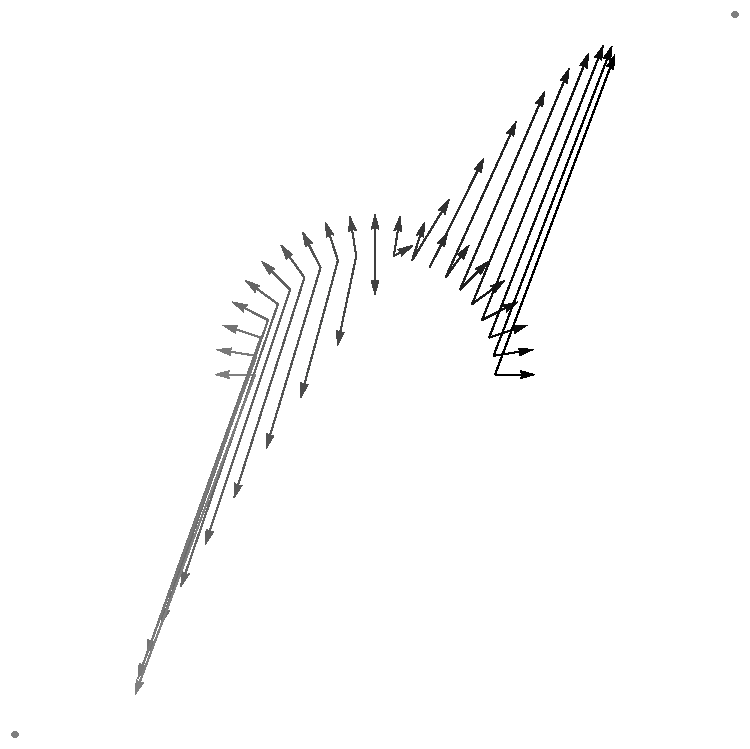
\includegraphics[width=0.44\linewidth]{Eigen2}
	\end{array} \] 

\begin{myexb}[\bd{b}]
	Given $\mtx{A} = \left[ \begin{array}{cc} 1 & 3 \\ 4 & 2 \end{array} \right]$, find all values for $\lambda$ such that the matrix equation \[ (\mtx{A} - \lambda \mtx{I})\vect{v} = \vect{0}\] has a solution other that other than $\vect{v} = \vect{0}$. These are the eigenvalues for \mtx{A}.
\end{myexb}

\begin{myexc}[\bd{c}]
	Given $\mtx{A} = \left[ \begin{array}{rrr} 2 & 0 & 0 \\ 3 & -1 & 0 \\ 3 & 0 & -1 \end{array} \right]$ has eigenvalues $\lambda_\vect{v} = 2$ and $\lambda_\vect{w} = -1$. 
	\begin{tabbing}
		\indent   i. \space  \= Describe the set of vectors \vect{v} such that \mtx{A}\vect{v} = 2\vect{v} \\
		\indent  ii. \> Describe the set of vectors \vect{w} such that \mtx{A}\vect{w} = -1\vect{w}  \\
	\end{tabbing}
\end{myexc}

\noindent \bd{Discussion Question 32.} If an eigenvector could be zero what would the corresponding eigenvalue be?

\vspace{.5cm}

\begin{theorem}
	For any  $n \times n$ matrix \mtx{A}, the set of eigenvectors corresponding to a given eigenvalue $\lambda$ becomes a subspace of $\mathbb{R}^n$ if you include  \bd{0}. 
\end{theorem}

\noindent \bd{Challenge 32.} Given matrix \mtx{A} has eigenvector \vect{v} with eigenvalue $\lambda$ and $k~\in~\mathbb{R}$. What can you say about the eigenvectors and eigenvalues of the matrix $k\mtx{A}$? What can you say about the eigenvectors and eigenvalues of the matrix $\mtx{A}^k$?  Does it matter what $k$ is?   

\vspace{.5cm}

\section{When an Eigenvalue is 0}    \label{When an Eigenvalue is 0}

\begin{myexa}[\bd{a}]
	Recall that if there are elementary matrices  $\mtx{E}_1$, $\mtx{E}_2$,...$\mtx{E}_k$  such that $\mtx{E}_k\cdots\mtx{E}_2\mtx{E}_1\mtx{A} = \mtx{I} $ then  $\mtx{A}^{-1}= \mtx{E}_k\cdots\mtx{E}_2\mtx{E}_1$. For  $\mtx{A} = \left[ \begin{array}{rrr}  3 & 0 & 1 \\ 0 & 2 & 1 \\ 1 & 1 & 1 \end{array} \right]$ find $\mtx{A}^{-1}$ by starting with $[\mtx{A}:\mtx{I}]$ then using the same elementary row operation on both sides to get $[\mtx{I}:\mtx{A}^{-1}]$.  Check your answer by computing $\mtx{A}^{-1}\mtx{A}$. 
\end{myexa} 

\noindent \bd{Discussion Question 33.} Can eigenvalues be zero? What would it mean if a vector's eigenvalue were zero?

\begin{myexb}[\bd{b}]
		Compute the eigenvalues and their corresponding eigenspaces for   $\mtx{A} = \left[ \begin{array}{rr}  2 & -4 \\ -3 & 6  \end{array} \right]$.
\end{myexb}

\begin{myexc}[\bd{c}]
		Compute the eigenvalues and their corresponding eigenspaces for  $\mtx{A} = \left[ \begin{array}{rrr} 1 & 1 & -1 \\ 1 & -1 & 1 \\ 1 & 1 & -1 \end{array} \right]$.
\end{myexc}

\begin{theorem}
	 An $n \times n$ matrices \mtx{A} is invertible if and only if none of its eigenvalues are zero.  
\end{theorem}
\vspace{-.3in}\hspace{5in}\begin{annotation}
	\endnote{ As an "if and only if" statement this proof will have two parts, set them up carefully. The definition, \mtx{A}v = $\lambda$\vect{v}, and "The Big Theorem" will be useful. }
\end{annotation}

\vspace{.5cm}

\noindent \bd{Challenge 33.} Given an invertible square matrix \mtx{A} with eigenvector \vect{v} and eigenvalue $\lambda$, show $\mtx{A}^{-1}$ also has eigenvector \vect{v}, but with eigenvalue $\frac{1}{\lambda}$. 

\vspace{.5cm}

\section{When Eigenvalues are Distinct}    \label{When Eigenvalues are Distinct}

\begin{myexa}[\bd{a}]
	Compute the eigenvalues and a representative eigenvector for   $\mtx{A} = \left[ \begin{array}{rr}  1 & 2 \\ 3 & -4  \end{array} \right]$ and for  $2\mtx{A} = \left[ \begin{array}{rr}  2 & 4 \\ 6 & -8  \end{array} \right]$. What do you notice?
\end{myexa} 

\noindent \bd{Discussion Question 34.} For a given eigenvalue can there be just one corresponding eigenvector? Usually books talk about eigenvectors as if there were just one, why doesn't this cause problems? 

\begin{myexb}[\bd{b}]
		Compute the eigenvalues and eigenvectors for   $\mtx{A} = \left[ \begin{array}{rr}  1 & 0 \\ 2 & 3  \end{array} \right]$ .
\end{myexb}

\begin{myexc}[\bd{c}]
	Compute the eigenvalues and eigenvectors for   $\mtx{A} = \left[ \begin{array}{rrr} 1 & 2 & 3 \\ 0 & 4 & 5 \\ 0 & 0 & 6 \end{array} \right]$.
\end{myexc}



\begin{theorem}
	Suppose \mtx{A} is a square matrix with eigenvectors \vect{v} and \vect{w}, and corresponding eigenvalues $\lambda_\vect{v}$ and $\lambda_\vect{w}$. If $\lambda_\vect{v}\ \neq \lambda_\vect{w}$ then \vect{v} and \vect{w} are linearly independent. 
\end{theorem}
\vspace{-.3in}\hspace{5in}\begin{annotation}
	\endnote{This theorem can be proved using any of the equivalent conditions for linearly independent. Each way will involve multiplying both sides of an equation by \mtx{A} and applying the definition of eigenvector, then combining the result with the original equation.  It will be important to note that, by definition, eigenvectors cannot be zero. }
\end{annotation}

\vspace{.5cm}

\noindent \bd{Challenge 34.} Given a square matrix \mtx{A} with three eigenvectors \vect{u}, \vect{v} and \vect{w}, having distinct corresponding eigenvalues $\lambda_\vect{u}$, $\lambda_\vect{v}$ and $\lambda_\vect{w}$, show \vect{u}, \vect{v} and \vect{w} are linearly independent. 

\vspace{.5cm}

\section{Diagonalization}    \label{Diagonalization}

\begin{myexa}[\bd{a}]
	Compute the following matrix products.
	\begin{tabbing}
		\indent   i. \space  \=  $\left[ \begin{array}{rrr} 1 & 2 & 3 \\ 4 & 5 & 6 \\ 7 & 8 & 9 \end{array} \right]\left[ \begin{array}{ccc} 10 & 0 & 0 \\ 0 & 100 & 0 \\ 0 & 0 & 1000 \end{array} \right]=$ \\
	\\
		\indent  ii. \>  $\left[ \begin{array}{ccc} 10 & 0 & 0 \\ 0 & 100 & 0 \\ 0 & 0 & 1000 \end{array} \right]\left[ \begin{array}{rrr} 1 & 2 & 3 \\ 4 & 5 & 6 \\ 7 & 8 & 9 \end{array} \right]=$  \\
	\end{tabbing}
\end{myexa} 

\begin{myexb}[\bd{b}]
	 Use that \vect{v_1} =(3,0,1), \vect{v_2} =(0,2,1) and \vect{v_3} =(1,1,1) are the eigenvectors corresponding to eigenvalues $\lambda_1 =0$, $\lambda_2=2$ and $\lambda_3=1$ for the matrix $\mtx{A} = \left[ \begin{array}{rrr} -2 & -3 & 6 \\ 2 & 5 & -6 \\ 0 & 1 & 0 \end{array} \right]$ to fill in the blanks below.
	 
	 
	$\left[ \begin{array}{rrr} -2 & -3 & 6 \\ 2 & 5 & -6 \\ 0 & 1 & 0 \end{array} \right]\left[ \begin{array}{ccc} \underline{\hspace{.2in} }  &  \underline{\hspace{.2in} } & \underline{\hspace{.2in} }  \\	 \underline{\hspace{.2in} }  &  \underline{\hspace{.2in} } & \underline{\hspace{.2in} } \\ \underline{\hspace{.2in} }  &  \underline{\hspace{.2in} } & \underline{\hspace{.2in} }\\
	\end{array} \right]   =  \left[ \begin{array}{ccc} \underline{\hspace{.2in} }  &  \underline{\hspace{.2in} } & \underline{\hspace{.2in} }  \\	 \underline{\hspace{.2in} }  &  \underline{\hspace{.2in} } & \underline{\hspace{.2in} } \\ \underline{\hspace{.2in} }  &  \underline{\hspace{.2in} } & \underline{\hspace{.2in} }\\
	\end{array} \right]\left[ \begin{array}{ccc} \underline{\hspace{.2in} }  &  \underline{\hspace{.2in} } & \underline{\hspace{.2in} }  \\	 \underline{\hspace{.2in} }  &  \underline{\hspace{.2in} } & \underline{\hspace{.2in} } \\ \underline{\hspace{.2in} }  &  \underline{\hspace{.2in} } & \underline{\hspace{.2in} }\\
	\end{array} \right]$ \\
	
and \\
	
	 $\left[ \begin{array}{rrr} -2 & -3 & 6 \\ 2 & 5 & -6 \\ 0 & 1 & 0 \end{array} \right]  = \left[ \begin{array}{ccc} \underline{\hspace{.2in} }  &  \underline{\hspace{.2in} } & \underline{\hspace{.2in} }  \\	 \underline{\hspace{.2in} }  &  \underline{\hspace{.2in} } & \underline{\hspace{.2in} } \\ \underline{\hspace{.2in} }  &  \underline{\hspace{.2in} } & \underline{\hspace{.2in} }\\
	 \end{array} \right]  \left[ \begin{array}{ccc} \underline{\hspace{.2in} }  &  0 & 0  \\	 0  &  \underline{\hspace{.2in} } & 0 \\ 0  &  0 & \underline{\hspace{.2in} }\\
	 \end{array} \right]\left[ \begin{array}{ccc} \underline{\hspace{.2in} }  &  \underline{\hspace{.2in} } & \underline{\hspace{.2in} }  \\	 \underline{\hspace{.2in} }  &  \underline{\hspace{.2in} } & \underline{\hspace{.2in} } \\ \underline{\hspace{.2in} }  &  \underline{\hspace{.2in} } & \underline{\hspace{.2in} }\\
	 \end{array} \right]$
\end{myexb}

\vspace{.5cm}

\begin{myexc}[\bd{c}]
	Given $\mtx{A} = \left[ \begin{array}{rr} 1 & -1  \\ 2 & 4  \end{array} \right]$, find invertible matrix \mtx{P} and diagonal matrix \mtx{D} such that $\mtx{A} = \mtx{P}\mtx{D}\mtx{P}^{-1}$ 
\end{myexc}


\begin{theorem}
	If an $n\times n$ matrix has n linearly independent eigenvectors then there exists an invertible matrix \mtx{P} and a diagonal matrix \mtx{D} such that: \[	\mtx{A} = \mtx{P }\mtx{D}\ \mtx{P}^{\ -1} \]
\end{theorem}

\vspace{.5cm}

\noindent \bd{Challenge 35.} 	If an $n\times n$ matrix \mtx{A} has n linearly independent eigenvectors then det(\mtx{A}) is the product of the n corresponding eigenvalues. 

\vspace{.5cm}

\noindent \bd{Discussion Question 35.} How would Theorem 35 help us efficiently compute $\mtx{A}^{100}$?


% \fi  % to omit ch3	

%%%%%%%%%%%%%%%%%%%%%%%%%%%%%%%%%%%%%%%%%%%%












%%%%%%%%%%%%%%%%%%%%%%%%%%%%%%%%%%%%%%%%%%%%%




%%%%%%%%%%%%%%%%%%%%%%%%%%%BEGIN REMOVAL {5} %%%%%%%%%%%%%%%%%%%%%%%%%%%%%%%%%
\backmatter

\begin{annotation}
\chapter{Notes to the Instructor}

\renewcommand\notesname{}
\vspace{-2cm}
\begingroup
%\setlength{\parindent}{0pt}% Don't know what this does.  DMC
\setlength{\parskip}{2ex}
\renewcommand{\enotesize}{\normalsize}

\theendnotes

\endgroup

\end{annotation}



%%%%%%%%%%%%%%%%%%%%%%%%%%%END REMOVAL {5} %%%%%%%%%%%%%%%%%%%%%%%%%%%%%%%%%

\end{document}
